% ----------------------------------------------------------------------
%
%                            TFMTesis.tex
%
%----------------------------------------------------------------------
%
% Este fichero contiene el "documento maestro" del documento. Lo único
% que hace es configurar el entorno LaTeX e incluir los ficheros .tex
% que contienen cada sección.
%
%----------------------------------------------------------------------
%
% Los ficheros necesarios para este documento son:
%
%       TeXiS/* : ficheros de la plantilla TeXiS.
%       Cascaras/* : ficheros con las partes del documento que no
%          son capítulos ni apéndices (portada, agradecimientos, etc.)
%       Capitulos/*.tex : capítulos de la tesis
%       Apendices/*.tex: apéndices de la tesis
%       constantes.tex: constantes LaTeX
%       config.tex : configuración de la "compilación" del documento
%       guionado.tex : palabras con guiones
%
% Para la bibliografía, además, se necesitan:
%
%       *.bib : ficheros con la información de las referencias
%
% ---------------------------------------------------------------------

\documentclass[11pt,a4paper,twoside]{book}

%
% Definimos  el   comando  \compilaCapitulo,  que   luego  se  utiliza
% (opcionalmente) en config.tex. Quedaría  mejor si también se definiera
% en  ese fichero,  pero por  el modo  en el  que funciona  eso  no es
% posible. Puedes consultar la documentación de ese fichero para tener
% más  información. Definimos también  \compilaApendice, que  tiene el
% mismo  cometido, pero  que se  utiliza para  compilar  únicamente un
% apéndice.
%
%
% Si  queremos   compilar  solo   una  parte  del   documento  podemos
% especificar mediante  \includeonly{...} qué ficheros  son los únicos
% que queremos  que se incluyan.  Esto  es útil por  ejemplo para sólo
% compilar un capítulo.
%
% El problema es que todos aquellos  ficheros que NO estén en la lista
% NO   se  incluirán...  y   eso  también   afecta  a   ficheros  de
% la plantilla...
%
% Total,  que definimos  una constante  con los  ficheros  que siempre
% vamos a querer compilar  (aquellos relacionados con configuración) y
% luego definimos \compilaCapitulo.
\newcommand{\ficherosBasicosTeXiS}{%
TeXiS/TeXiS_pream,TeXiS/TeXiS_cab,TeXiS/TeXiS_bib,TeXiS/TeXiS_cover%
}
\newcommand{\ficherosBasicosTexto}{%
constantes,guionado,Cascaras/bibliografia,config%
}
\newcommand{\compilaCapitulo}[1]{%
\includeonly{\ficherosBasicosTeXiS,\ficherosBasicosTexto,Capitulos/#1}%
}

\newcommand{\compilaApendice}[1]{%
\includeonly{\ficherosBasicosTeXiS,\ficherosBasicosTexto,Apendices/#1}%
}

%- - - - - - - - - - - - - - - - - - - - - - - - - - - - - - - - - - -
%            Preámbulo del documento. Configuraciones varias
%- - - - - - - - - - - - - - - - - - - - - - - - - - - - - - - - - - -

% Define  el  tipo  de  compilación que  estamos  haciendo.   Contiene
% definiciones  de  constantes que  cambian  el  comportamiento de  la
% compilación. Debe incluirse antes del paquete TeXiS/TeXiS.sty
%---------------------------------------------------------------------
%
%                          config.tex
%
%---------------------------------------------------------------------
%
% Contiene la  definición de constantes  que determinan el modo  en el
% que se compilará el documento.
%
%---------------------------------------------------------------------
%
% En concreto, podemos  indicar si queremos "modo release",  en el que
% no  aparecerán  los  comentarios  (creados  mediante  \com{Texto}  o
% \comp{Texto}) ni los "por  hacer" (creados mediante \todo{Texto}), y
% sí aparecerán los índices. El modo "debug" (o mejor dicho en modo no
% "release" muestra los índices  (construirlos lleva tiempo y son poco
% útiles  salvo  para   la  versión  final),  pero  sí   el  resto  de
% anotaciones.
%
% Si se compila con LaTeX (no  con pdflatex) en modo Debug, también se
% muestran en una esquina de cada página las entradas (en el índice de
% palabras) que referencian  a dicha página (consulta TeXiS_pream.tex,
% en la parte referente a show).
%
% El soporte para  el índice de palabras en  TeXiS es embrionario, por
% lo  que no  asumas que  esto funcionará  correctamente.  Consulta la
% documentación al respecto en TeXiS_pream.tex.
%
%
% También  aquí configuramos  si queremos  o  no que  se incluyan  los
% acrónimos  en el  documento final  en la  versión release.  Para eso
% define (o no) la constante \acronimosEnRelease.
%
% Utilizando \compilaCapitulo{nombre}  podemos también especificar qué
% capítulo(s) queremos que se compilen. Si no se pone nada, se compila
% el documento  completo.  Si se pone, por  ejemplo, 01Introduccion se
% compilará únicamente el fichero Capitulos/01Introduccion.tex
%
% Para compilar varios  capítulos, se separan sus nombres  con comas y
% no se ponen espacios de separación.
%
% En realidad  la macro \compilaCapitulo  está definida en  el fichero
% principal tesis.tex.
%
%---------------------------------------------------------------------


% Comentar la línea si no se compila en modo release.
% TeXiS hará el resto.
% ¡¡¡Si cambias esto, haz un make clean antes de recompilar!!!
\def\release{1}


% Descomentar la linea si se quieren incluir los
% acrónimos en modo release (en modo debug
% no se incluirán nunca).
% ¡¡¡Si cambias esto, haz un make clean antes de recompilar!!!
%\def\acronimosEnRelease{1}


% Descomentar la línea para establecer el capítulo que queremos
% compilar

% \compilaCapitulo{01Introduccion}
% \compilaCapitulo{02EstructuraYGeneracion}
% \compilaCapitulo{03Edicion}
% \compilaCapitulo{04Imagenes}
% \compilaCapitulo{05Bibliografia}
% \compilaCapitulo{06Makefile}

% \compilaApendice{01AsiSeHizo}

% Variable local para emacs, para  que encuentre el fichero maestro de
% compilación y funcionen mejor algunas teclas rápidas de AucTeX
%%%
%%% Local Variables:
%%% mode: latex
%%% TeX-master: "./Tesis.tex"
%%% End:


% Paquete de la plantilla
\usepackage{TeXiS/TeXiS}

% Incluimos el fichero con comandos de constantes
%---------------------------------------------------------------------
%
%                          constantes.tex
%
%---------------------------------------------------------------------
%
% Fichero que  declara nuevos comandos LaTeX  sencillos realizados por
% comodidad en la escritura de determinadas palabras
%
%---------------------------------------------------------------------

%%%%%%%%%%%%%%%%%%%%%%%%%%%%%%%%%%%%%%%%%%%%%%%%%%%%%%%%%%%%%%%%%%%%%%
% Comando: 
%
%       \titulo
%
% Resultado: 
%
% Escribe el título del documento.
%%%%%%%%%%%%%%%%%%%%%%%%%%%%%%%%%%%%%%%%%%%%%%%%%%%%%%%%%%%%%%%%%%%%%%
\def\titulo{\textsc{TeXiS}: Una plantilla de \LaTeX\
  para Tesis y otros documentos}

%%%%%%%%%%%%%%%%%%%%%%%%%%%%%%%%%%%%%%%%%%%%%%%%%%%%%%%%%%%%%%%%%%%%%%
% Comando: 
%
%       \autor
%
% Resultado: 
%
% Escribe el autor del documento.
%%%%%%%%%%%%%%%%%%%%%%%%%%%%%%%%%%%%%%%%%%%%%%%%%%%%%%%%%%%%%%%%%%%%%%
\def\autor{Marco Antonio y Pedro Pablo G\'omez Mart\'in}

% Variable local para emacs, para  que encuentre el fichero maestro de
% compilación y funcionen mejor algunas teclas rápidas de AucTeX

%%%
%%% Local Variables:
%%% mode: latex
%%% TeX-master: "tesis.tex"
%%% End:


% Sacamos en el log de la compilación el copyright
%\typeout{Copyright Marco Antonio and Pedro Pablo Gomez Martin}

%
% "Metadatos" para el PDF
%
\ifpdf\hypersetup{%
    pdftitle = {\titulo},
    pdfsubject = {Plantilla de Tesis},
    pdfkeywords = {Plantilla, LaTeX, tesis, trabajo de
      investigación, trabajo de Master},
    pdfauthor = {\textcopyright\ \autor},
    pdfcreator = {\LaTeX\ con el paquete \flqq hyperref\frqq},
    pdfproducer = {pdfeTeX-0.\the\pdftexversion\pdftexrevision},
    }
    \pdfinfo{/CreationDate (\today)}
\fi


%- - - - - - - - - - - - - - - - - - - - - - - - - - - - - - - - - - -
%                        Documento
%- - - - - - - - - - - - - - - - - - - - - - - - - - - - - - - - - - -
\begin{document}

% Incluimos el  fichero de definición de guionado  de algunas palabras
% que LaTeX no ha dividido como debería
%----------------------------------------------------------------
%
%                          guionado.tex
%
%----------------------------------------------------------------
%
% Fichero con algunas divisiones de palabras que LaTeX no
% hace correctamente si no se le da alguna ayuda.
%
%----------------------------------------------------------------

\hyphenation{
% a
abs-trac-to
abs-trac-tos
abs-trac-ta
abs-trac-tas
ac-tua-do-res
a-gra-de-ci-mien-tos
ana-li-za-dor
an-te-rio-res
an-te-rior-men-te
apa-rien-cia
a-pro-pia-do
a-pro-pia-dos
a-pro-pia-da
a-pro-pia-das
a-pro-ve-cha-mien-to
a-que-llo
a-que-llos
a-que-lla
a-que-llas
a-sig-na-tu-ra
a-sig-na-tu-ras
a-so-cia-da
a-so-cia-das
a-so-cia-do
a-so-cia-dos
au-to-ma-ti-za-do
% b
batch
bi-blio-gra-fía
bi-blio-grá-fi-cas
bien
bo-rra-dor
boo-l-ean-expr
% c
ca-be-ce-ra
call-me-thod-ins-truc-tion
cas-te-lla-no
cir-cuns-tan-cia
cir-cuns-tan-cias
co-he-ren-te
co-he-ren-tes
co-he-ren-cia
co-li-bri
co-men-ta-rio
co-mer-cia-les
co-no-ci-mien-to
cons-cien-te
con-si-de-ra-ba
con-si-de-ra-mos
con-si-de-rar-se
cons-tan-te
cons-trucción
cons-tru-ye
cons-tru-ir-se
con-tro-le
co-rrec-ta-men-te
co-rres-pon-den
co-rres-pon-dien-te
co-rres-pon-dien-tes
co-ti-dia-na
co-ti-dia-no
crean
cris-ta-li-zan
cu-rri-cu-la
cu-rri-cu-lum
cu-rri-cu-lar
cu-rri-cu-la-res
% d
de-di-ca-do
de-di-ca-dos
de-di-ca-da
de-di-ca-das
de-rro-te-ro
de-rro-te-ros
de-sa-rro-llo
de-sa-rro-llos
de-sa-rro-lla-do
de-sa-rro-lla-dos
de-sa-rro-lla-da
de-sa-rro-lla-das
de-sa-rro-lla-dor
de-sa-rro-llar
des-cri-bi-re-mos
des-crip-ción
des-crip-cio-nes
des-cri-to
des-pués
de-ta-lla-do
de-ta-lla-dos
de-ta-lla-da
de-ta-lla-das
di-a-gra-ma
di-a-gra-mas
di-se-ños
dis-po-ner
dis-po-ni-bi-li-dad
do-cu-men-ta-da
do-cu-men-to
do-cu-men-tos
% e
edi-ta-do
e-du-ca-ti-vo
e-du-ca-ti-vos
e-du-ca-ti-va
e-du-ca-ti-vas
e-la-bo-ra-do
e-la-bo-ra-dos
e-la-bo-ra-da
e-la-bo-ra-das
es-co-llo
es-co-llos
es-tu-dia-do
es-tu-dia-dos
es-tu-dia-da
es-tu-dia-das
es-tu-dian-te
e-va-lua-cio-nes
e-va-lua-do-res
exis-ten-tes
exhaus-ti-va
ex-pe-rien-cia
ex-pe-rien-cias
% f
for-ma-li-za-do
% g
ge-ne-ra-ción
ge-ne-ra-dor
ge-ne-ra-do-res
ge-ne-ran
% h
he-rra-mien-ta
he-rra-mien-tas
% i
i-dio-ma
i-dio-mas
im-pres-cin-di-ble
im-pres-cin-di-bles
in-de-xa-do
in-de-xa-dos
in-de-xa-da
in-de-xa-das
in-di-vi-dual
in-fe-ren-cia
in-fe-ren-cias
in-for-ma-ti-ca
in-gre-dien-te
in-gre-dien-tes
in-me-dia-ta-men-te
ins-ta-la-do
ins-tan-cias
% j
% k
% l
len-gua-je
li-be-ra-to-rio
li-be-ra-to-rios
li-be-ra-to-ria
li-be-ra-to-rias
li-mi-ta-do
li-te-ra-rio
li-te-ra-rios
li-te-ra-ria
li-te-ra-rias
lo-tes
% m
ma-ne-ra
ma-nual
mas-que-ra-de
ma-yor
me-mo-ria
mi-nis-te-rio
mi-nis-te-rios
mo-de-lo
mo-de-los
mo-de-la-do
mo-du-la-ri-dad
mo-vi-mien-to
% n
na-tu-ral
ni-vel
nues-tro
% o
obs-tan-te
o-rien-ta-do
o-rien-ta-dos
o-rien-ta-da
o-rien-ta-das
% p
pa-ra-le-lo
pa-ra-le-la
par-ti-cu-lar
par-ti-cu-lar-men-te
pe-da-gó-gi-ca
pe-da-gó-gi-cas
pe-da-gó-gi-co
pe-da-gó-gi-cos
pe-rio-di-ci-dad
per-so-na-je
plan-te-a-mien-to
plan-te-a-mien-tos
po-si-ción
pre-fe-ren-cia
pre-fe-ren-cias
pres-cin-di-ble
pres-cin-di-bles
pri-me-ra
pro-ble-ma
pro-ble-mas
pró-xi-mo
pu-bli-ca-cio-nes
pu-bli-ca-do
% q
% r
rá-pi-da
rá-pi-do
ra-zo-na-mien-to
ra-zo-na-mien-tos
re-a-li-zan-do
re-fe-ren-cia
re-fe-ren-cias
re-fe-ren-cia-da
re-fe-ren-cian
re-le-van-tes
re-pre-sen-ta-do
re-pre-sen-ta-dos
re-pre-sen-ta-da
re-pre-sen-ta-das
re-pre-sen-tar-lo
re-qui-si-to
re-qui-si-tos
res-pon-der
res-pon-sa-ble
% s
se-pa-ra-do
si-guien-do
si-guien-te
si-guien-tes
si-guie-ron
si-mi-lar
si-mi-la-res
si-tua-ción
% t
tem-pe-ra-ments
te-ner
trans-fe-ren-cia
trans-fe-ren-cias
% u
u-sua-rio
Unreal-Ed
% v
va-lor
va-lo-res
va-rian-te
ver-da-de-ro
ver-da-de-ros
ver-da-de-ra
ver-da-de-ras
ver-da-de-ra-men-te
ve-ri-fi-ca
% w
% x
% y
% z
}
% Variable local para emacs, para que encuentre el fichero
% maestro de compilación
%%%
%%% Local Variables:
%%% mode: latex
%%% TeX-master: "./Tesis.tex"
%%% End:


% Marcamos  el inicio  del  documento para  la  numeración de  páginas
% (usando números romanos para esta primera fase).
\frontmatter
\pagestyle{empty}

%---------------------------------------------------------------------
%
%                          configCover.tex
%
%---------------------------------------------------------------------
%
% cover.tex
% Copyright 2009 Marco Antonio Gomez-Martin, Pedro Pablo Gomez-Martin
%
% This file belongs to the TeXiS manual, a LaTeX template for writting
% Thesis and other documents. The complete last TeXiS package can
% be obtained from http://gaia.fdi.ucm.es/projects/texis/
%
% Although the TeXiS template itself is distributed under the 
% conditions of the LaTeX Project Public License
% (http://www.latex-project.org/lppl.txt), the manual content
% uses the CC-BY-SA license that stays that you are free:
%
%    - to share & to copy, distribute and transmit the work
%    - to remix and to adapt the work
%
% under the following conditions:
%
%    - Attribution: you must attribute the work in the manner
%      specified by the author or licensor (but not in any way that
%      suggests that they endorse you or your use of the work).
%    - Share Alike: if you alter, transform, or build upon this
%      work, you may distribute the resulting work only under the
%      same, similar or a compatible license.
%
% The complete license is available in
% http://creativecommons.org/licenses/by-sa/3.0/legalcode
%
%---------------------------------------------------------------------
%
% Fichero que contiene la configuración de la portada y de la 
% primera hoja del documento.
%
%---------------------------------------------------------------------


% Pueden configurarse todos los elementos del contenido de la portada
% utilizando comandos.

%%%%%%%%%%%%%%%%%%%%%%%%%%%%%%%%%%%%%%%%%%%%%%%%%%%%%%%%%%%%%%%%%%%%%%
% Título del documento:
% \tituloPortada{titulo}
% Nota:
% Si no se define se utiliza el del \titulo. Este comando permite
% cambiar el título de forma que se especifiquen dónde se quieren
% los retornos de carro cuando se utilizan fuentes grandes.
%%%%%%%%%%%%%%%%%%%%%%%%%%%%%%%%%%%%%%%%%%%%%%%%%%%%%%%%%%%%%%%%%%%%%%
\tituloPortada{%
IRIS: Asistente virtual para la redacción personalizada de correos electrónicos
}


%%%%%%%%%%%%%%%%%%%%%%%%%%%%%%%%%%%%%%%%%%%%%%%%%%%%%%%%%%%%%%%%%%%%%%
% Título del documento en inglés:
% \tituloPortadaEng{titulo}
% Nota:
% Si no se define se utiliza el del \titulo. Este comando permite
% cambiar el título de forma que se especifiquen dónde se quieren
% los retornos de carro cuando se utilizan fuentes grandes.
%%%%%%%%%%%%%%%%%%%%%%%%%%%%%%%%%%%%%%%%%%%%%%%%%%%%%%%%%%%%%%%%%%%%%%
\tituloPortadaEng{%
IRIS: Virtual Assistant for Personalized Email Writing
}

%%%%%%%%%%%%%%%%%%%%%%%%%%%%%%%%%%%%%%%%%%%%%%%%%%%%%%%%%%%%%%%%%%%%%%
% Autor del documento:
% \autorPortada{Nombre}
% Se utiliza en la portada y en el valor por defecto del
% primer subtítulo de la segunda portada.
%%%%%%%%%%%%%%%%%%%%%%%%%%%%%%%%%%%%%%%%%%%%%%%%%%%%%%%%%%%%%%%%%%%%%%
\autorPortada{Carlos Moreno Morera}

%%%%%%%%%%%%%%%%%%%%%%%%%%%%%%%%%%%%%%%%%%%%%%%%%%%%%%%%%%%%%%%%%%%%%%
% Fecha de publicación:
% \fechaPublicacion{Fecha}
% Puede ser vacío. Aparece en la última línea de ambas portadas
%%%%%%%%%%%%%%%%%%%%%%%%%%%%%%%%%%%%%%%%%%%%%%%%%%%%%%%%%%%%%%%%%%%%%%
% Descomentar para que ponga siempre la fecha actual
%\fechaPublicacion{\today}
\fechaPublicacion{\today}

%%%%%%%%%%%%%%%%%%%%%%%%%%%%%%%%%%%%%%%%%%%%%%%%%%%%%%%%%%%%%%%%%%%%%%
% Imagen de la portada (y escala)
% \imagenPortada{Fichero}
% \escalaImagenPortada{Numero}
% Si no se especifica, se utiliza la imagen TODO.pdf
%%%%%%%%%%%%%%%%%%%%%%%%%%%%%%%%%%%%%%%%%%%%%%%%%%%%%%%%%%%%%%%%%%%%%%
% imagen en blanco y negro
%\imagenPortada{Imagenes/Vectorial/escudoUCM}
%imagen en color
\imagenPortada{Imagenes/Bitmap/escudoUCMcolor}
\escalaImagenPortada{.2}

%%%%%%%%%%%%%%%%%%%%%%%%%%%%%%%%%%%%%%%%%%%%%%%%%%%%%%%%%%%%%%%%%%%%%%
% Tipo de documento.
% \tipoDocumento{Tipo}
% Para el texto justo debajo del escudo.
% Si no se indica, se utiliza "TESIS DOCTORAL".
%%%%%%%%%%%%%%%%%%%%%%%%%%%%%%%%%%%%%%%%%%%%%%%%%%%%%%%%%%%%%%%%%%%%%%
\tipoDocumento{Trabajo de Fin de Máster}

%%%%%%%%%%%%%%%%%%%%%%%%%%%%%%%%%%%%%%%%%%%%%%%%%%%%%%%%%%%%%%%%%%%%%%
% Institución/departamento asociado al documento.
% \institucion{Nombre}
% Puede tener varias líneas. Se utiliza en las dos portadas.
% Si no se indica aparecerá vacío.
%%%%%%%%%%%%%%%%%%%%%%%%%%%%%%%%%%%%%%%%%%%%%%%%%%%%%%%%%%%%%%%%%%%%%%
\institucion{%
Máster en Data Science y Big Data\\[0.2em]
U-Tad
}

%%%%%%%%%%%%%%%%%%%%%%%%%%%%%%%%%%%%%%%%%%%%%%%%%%%%%%%%%%%%%%%%%%%%%%
% Director del trabajo.
% \directorPortada{Nombre}
% Se utiliza para el valor por defecto del segundo subtítulo, donde
% se indica quién es el director del trabajo.
% Si se fuerza un subtítulo distinto, no hace falta definirlo.
%%%%%%%%%%%%%%%%%%%%%%%%%%%%%%%%%%%%%%%%%%%%%%%%%%%%%%%%%%%%%%%%%%%%%%
\directorPortada{Carlos Rodríguez Abellán}


%%%%%%%%%%%%%%%%%%%%%%%%%%%%%%%%%%%%%%%%%%%%%%%%%%%%%%%%%%%%%%%%%%%%%%
% Colaborador en la dirección del trabajo.
% \colaboradorPortada{Nombre}
% Se utiliza para el valor por defecto del segundo subtítulo, donde
% se indica quién es el colaborador en la dirección del trabajo.
% Si se fuerza un subtítulo distinto, no hace falta definirlo.
%%%%%%%%%%%%%%%%%%%%%%%%%%%%%%%%%%%%%%%%%%%%%%%%%%%%%%%%%%%%%%%%%%%%%%
%\colaboradorPortada{\textcolor{red}{Colaborador 1\\Colaborador 2}}


%%%%%%%%%%%%%%%%%%%%%%%%%%%%%%%%%%%%%%%%%%%%%%%%%%%%%%%%%%%%%%%%%%%%%%
% Texto del primer subtítulo de la segunda portada.
% \textoPrimerSubtituloPortada{Texto}
% Para configurar el primer "texto libre" de la segunda portada.
% Si no se especifica se indica "Memoria que presenta para optar al
% título de Doctor en Informática" seguido del \autorPortada.
%%%%%%%%%%%%%%%%%%%%%%%%%%%%%%%%%%%%%%%%%%%%%%%%%%%%%%%%%%%%%%%%%%%%%%
\textoPrimerSubtituloPortada{%
\textbf{Trabajo de Fin de Máster en Data Science y Big Data}  \\ [0.3em]
}

%%%%%%%%%%%%%%%%%%%%%%%%%%%%%%%%%%%%%%%%%%%%%%%%%%%%%%%%%%%%%%%%%%%%%%
% Texto del segundo subtítulo de la segunda portada.
% \textoSegundoSubtituloPortada{Texto}
% Para configurar el segundo "texto libre" de la segunda portada.
% Si no se especifica se indica "Dirigida por el Doctor" seguido
% del \directorPortada.
%%%%%%%%%%%%%%%%%%%%%%%%%%%%%%%%%%%%%%%%%%%%%%%%%%%%%%%%%%%%%%%%%%%%%%
\textoSegundoSubtituloPortada{%
\textbf{Convocatoria: }\textit{Octubre \the\year}
}

%%%%%%%%%%%%%%%%%%%%%%%%%%%%%%%%%%%%%%%%%%%%%%%%%%%%%%%%%%%%%%%%%%%%%%
% \explicacionDobleCara
% Si se utiliza, se aclara que el documento está preparado para la
% impresión a doble cara.
%%%%%%%%%%%%%%%%%%%%%%%%%%%%%%%%%%%%%%%%%%%%%%%%%%%%%%%%%%%%%%%%%%%%%%
%\explicacionDobleCara

%%%%%%%%%%%%%%%%%%%%%%%%%%%%%%%%%%%%%%%%%%%%%%%%%%%%%%%%%%%%%%%%%%%%%%
% \isbn
% Si se utiliza, aparecerá el ISBN detrás de la segunda portada.
%%%%%%%%%%%%%%%%%%%%%%%%%%%%%%%%%%%%%%%%%%%%%%%%%%%%%%%%%%%%%%%%%%%%%%
%\isbn{978-84-692-7109-4}


%%%%%%%%%%%%%%%%%%%%%%%%%%%%%%%%%%%%%%%%%%%%%%%%%%%%%%%%%%%%%%%%%%%%%%
% \copyrightInfo
% Si se utiliza, aparecerá información de los derechos de copyright
% detrás de la segunda portada.
%%%%%%%%%%%%%%%%%%%%%%%%%%%%%%%%%%%%%%%%%%%%%%%%%%%%%%%%%%%%%%%%%%%%%%
%\copyrightInfo{\autor}


%%
%% Creamos las portadas
%%
\makeCover

% Variable local para emacs, para que encuentre el fichero
% maestro de compilación
%%%
%%% Local Variables:
%%% mode: latex
%%% TeX-master: "../Tesis.tex"
%%% End:

%\chapter*{Autorización de difusión}

   
El abajo firmante, matriculado en el Máster en Ingeniería en Informática de la Facultad de Informática, autoriza a la Universidad Complutense de Madrid (UCM) a difundir y utilizar con fines académicos, no comerciales y mencionando expresamente a su autor el presente Trabajo Fin de Máster: ``TITULO DEL TRABAJO'', realizado durante el curso académico CURSO bajo la dirección de DIRECTORES en el Departamento de XXXXXXXXXXXXXXXXXXXXXXXX, y a la Biblioteca de la UCM a depositarlo en el Archivo Institucional E-Prints Complutense con el objeto de incrementar la difusión, uso e impacto del trabajo en Internet y garantizar su preservación y acceso a largo plazo.

\vspace{5cm}

% +--------------------------------------------------------------------+
% | On the line below, replace "Enter Your Name" with your name
% | Use the same form of your name as it appears on your title page.
% | Use mixed case, for example, Lori Goetsch.
% +--------------------------------------------------------------------+
\begin{center}
	\large Nombre Del Alumno\\
	
	\vspace{0.5cm}
	
	% +--------------------------------------------------------------------+
	% | On the line below, replace Fecha
	% |
	% +--------------------------------------------------------------------+
	
	\today\\
	
\end{center}

% +--------------------------------------------------------------------+
% | Dedication Page (Optional)
% +--------------------------------------------------------------------+

\chapter*{Dedicatoria}

\begin{flushright}
\begin{minipage}[c]{8.5cm}
\flushright{\textit{A mi madre y mi padre}}
\end{minipage}
\end{flushright}
%% +--------------------------------------------------------------------+
% | Acknowledgements Page (Optional)                                   |
% +--------------------------------------------------------------------+

\chapter*{Agradecimientos}

A Guillermo, por el tiempo empleado en hacer estas plantillas. A Adrián, Enrique y Nacho, por sus comentarios para mejorar lo que hicimos. Y a Narciso, a quien no le ha hecho falta el Anillo Único para coordinarnos a todos.












\chapter*{Resumen}

\section*{\tituloPortadaVal}

Un resumen en castellano de media página, incluyendo el título en castellano. A continuación, se escribirá una lista de no más de 10 palabras clave.


\section*{Palabras clave}
   
\noindent Máximo 10 palabras clave separadas por comas

   



%\begin{otherlanguage}{english}
%\chapter*{Abstract}

\section*{\tituloPortadaEngVal}

An abstract in English, half a page long, including the title in English. Below, a list with no more than 10 keywords.


\section*{Keywords}

\noindent 10 keywords max., separated by commas.




% Si el trabajo se escribe en inglés, comentar esta línea y descomentar
% otra igual que hay justo antes de \end{document}
%\end{otherlanguage}

\ifx\generatoc\undefined
\else
%---------------------------------------------------------------------
%
%                          TeXiS_toc.tex
%
%---------------------------------------------------------------------
%
% TeXiS_toc.tex
% Copyright 2009 Marco Antonio Gomez-Martin, Pedro Pablo Gomez-Martin
%
% This file belongs to TeXiS, a LaTeX template for writting
% Thesis and other documents. The complete last TeXiS package can
% be obtained from http://gaia.fdi.ucm.es/projects/texis/
%
% This work may be distributed and/or modified under the
% conditions of the LaTeX Project Public License, either version 1.3
% of this license or (at your option) any later version.
% The latest version of this license is in
%   http://www.latex-project.org/lppl.txt
% and version 1.3 or later is part of all distributions of LaTeX
% version 2005/12/01 or later.
%
% This work has the LPPL maintenance status `maintained'.
% 
% The Current Maintainers of this work are Marco Antonio Gomez-Martin
% and Pedro Pablo Gomez-Martin
%
%---------------------------------------------------------------------
%
% Contiene  los  comandos  para  generar los  índices  del  documento,
% entendiendo por índices las tablas de contenidos.
%
% Genera  el  índice normal  ("tabla  de  contenidos"),  el índice  de
% figuras y el de tablas. También  crea "marcadores" en el caso de que
% se esté compilando con pdflatex para que aparezcan en el PDF.
%
%---------------------------------------------------------------------


% Primero un poquito de configuración...


% Pedimos que inserte todos los epígrafes hasta el nivel \subsection en
% la tabla de contenidos.
\setcounter{tocdepth}{2} 

% Le  pedimos  que nos  numere  todos  los  epígrafes hasta  el  nivel
% \subsubsection en el cuerpo del documento.
\setcounter{secnumdepth}{3} 


% Creamos los diferentes índices.

% Lo primero un  poco de trabajo en los marcadores  del PDF. No quiero
% que  salga una  entrada  por cada  índice  a nivel  0...  si no  que
% aparezca un marcador "Índices", que  tenga dentro los otros tipos de
% índices.  Total, que creamos el marcador "Índices".
% Antes de  la creación  de los índices,  se añaden los  marcadores de
% nivel 1.

\ifpdf
   \pdfbookmark{Índices}{indices}
\fi

% Tabla de contenidos.
%
% La  inclusión  de '\tableofcontents'  significa  que  en la  primera
% pasada  de  LaTeX  se  crea   un  fichero  con  extensión  .toc  con
% información sobre la tabla de contenidos (es conceptualmente similar
% al  .bbl de  BibTeX, creo).  En la  segunda ejecución  de  LaTeX ese
% documento se utiliza para  generar la verdadera página de contenidos
% usando la  información sobre los  capítulos y demás guardadas  en el
% .toc
\ifpdf
   \pdfbookmark[1]{Tabla de Contenidos}{tabla de contenidos}
\fi

\cabeceraEspecial{\'Indice}

\tableofcontents

\newpage 

% Índice de figuras
%
% La idea es semejante que para  el .toc del índice, pero ahora se usa
% extensión .lof (List Of Figures) con la información de las figuras.

\ifpdf
   \pdfbookmark[1]{Índice de figuras}{indice de figuras}
\fi

\cabeceraEspecial{\'Indice de figuras}

\listoffigures

\newpage

% Índice de tablas
% Como antes, pero ahora .lot (List Of Tables)

\ifpdf
   \pdfbookmark[1]{Índice de tablas}{indice de tablas}
\fi

\cabeceraEspecial{\'Indice de tablas}

\listoftables

\newpage

% Variable local para emacs, para  que encuentre el fichero maestro de
% compilación y funcionen mejor algunas teclas rápidas de AucTeX

%%%
%%% Local Variables:
%%% mode: latex
%%% TeX-master: "../Tesis.tex"
%%% End:

\fi

% Marcamos el  comienzo de  los capítulos (para  la numeración  de las
% páginas) y ponemos la cabecera normal
\mainmatter

\pagestyle{fancy}
\restauraCabecera


\chapter{Introducción}
\label{cap:introduccion}

\chapterquote{Frase célebre dicha por alguien inteligente}{Autor}


El estudiante elaborará una memoria descriptiva del trabajo realizado, con una \textbf{extensión mínima recomendada de 50 páginas} incluyendo al menos una introducción, objetivos y plan de trabajo, resultados con una discusión crítica y razonada de los mismos, conclusiones y bibliografía empleada en la elaboración de la memoria.

La memoria se puede redactar en castellano o en inglés, pero en el primer caso la introducción y las conclusiones de la memoria tienen que traducirse también al inglés y aparecerán como capítulos \textbf{al final de la memoria}. En ambos casos, el título de la memoria aparecerá en castellano y en inglés.

Además del cuerpo principal describiendo el trabajo realizado, la memoria contendrá los siguientes elementos, que no computarán para el cálculo de la extensión mínima del trabajo:

\begin{itemize}
\item un resumen en inglés de media página, incluyendo el título en inglés,
\item ese mismo resumen en castellano, incluyendo el título en castellano,
\item una lista de no más de 10 palabras clave en inglés,
\item esa misma lista en castellano,
\item un índice de contenidos, y
\item una bibliografía.
\end{itemize}

La portada de la memoria deberá contener la siguiente información:

\begin{itemize}
\item "Máster en NOMBRE DEL MÁSTER, Facultad de Informática, Universidad Complutense de Madrid"
\item Título
\item Autor
\item Director(es)
\item Colaborador externo de dirección, si lo hay
\item Curso académico
\item Solo en la versión final: convocatoria y calificación obtenida
\end{itemize}

Para facilitar la escritura de la memoria siguiendo esta estructura, el estudiante podrá usar las plantillas en LaTeX o Word preparadas al efecto y publicadas en la página web del máster correspondiente.

Todo el material no original, ya sea texto o figuras, deberá ser convenientemente citado y referenciado. En el caso de material complementario se deben respetar las licencias y copyrights asociados al software y hardware que se emplee. En caso contrario no se autorizará la defensa, sin menoscabo de otras acciones que correspondan.


\section{Motivación}
Introducción al tema del TFM.


\section{Objetivos}
Descripción de los objetivos del trabajo.


\section{Plan de trabajo}
Aquí se describe el plan de trabajo a seguir para la consecución de los objetivos descritos en el apartado anterior.



\section{Explicaciones adicionales sobre el uso de esta plantilla}
Si quieres cambiar el \textbf{estilo del título} de los capítulos, edita \verb|TeXiS\TeXiS_pream.tex| y comenta la línea \verb|\usepackage[Lenny]{fncychap}| para dejar el estilo básico de \LaTeX.

Si no te gusta que no haya \textbf{espacios entre párrafos} y quieres dejar un pequeño espacio en blanco, no metas saltos de línea (\verb|\\|) al final de los párrafos. En su lugar, busca el comando  \verb|\setlength{\parskip}{0.2ex}| en \verb|TeXiS\TeXiS_pream.tex| y aumenta el valor de $0.2ex$ a, por ejemplo, $1ex$.

TFMTeXiS se ha elaborado a partir de la plantilla de TeXiS\footnote{\url{http://gaia.fdi.ucm.es/research/texis/}}, creada por Marco Antonio y Pedro Pablo Gómez Martín para escribir su tesis doctoral. Para explicaciones más extensas y detalladas sobre cómo usar esta plantilla, recomendamos la lectura del documento \texttt{TeXiS-Manual-1.0.pdf} que acompaña a esta plantilla.

El siguiente texto se genera con el comando \verb|\lipsum[2-20]| que viene a continuación en el fichero .tex. El único propósito es mostrar el aspecto de las páginas usando esta plantilla. Quita este comando y, si quieres, comenta o elimina el paquete \textit{lipsum} al final de \verb|TeXiS\TeXiS_pream.tex|

\subsection{Texto de prueba}


\lipsum[2-20]
\chapter{Estado de la Cuestión}
\label{cap:estadoDeLaCuestion}

\chapterquote{Quien controla el presente controla el pasado y quien controla el pasado controlará el futuro.}{1984 - George Orwell (1949)}

Como se ha explicado en el capítulo anterior, el objetivo de este trabajo es el de desarrollar un sistema de generación de lenguaje natural capaz de, dada una representación semántica de lo que se quiere transmitir, redactar un correo electrónico completo. El primer paso para conseguir esta meta es entender en qué consiste la estructura de un correo electrónico y cómo es su formato, ya que el corpus del que se parte consta de e-mails reales extraídos de un servidor de mensajes. Por ello, en la sección \ref{s:email} se introducen los conceptos básicos, así como datos acerca de la utilización actual de este método de comunicación que demuestran la utilidad de contar con una aplicación que sea capaz de generarlos automáticamente. En concreto, se entrará en detalle de los principales protocolos que describen el formato de los e-mails (protocolo MIME explicado en la sección \ref{ss:mime}), cómo se mandan entre servidores (protocolo SMTP que se presenta en el apartado \ref{ss:smtp}) y cómo el usuario final los recibe y consulta (protocolos POP e IMAP desarrollados a lo largo de las secciones \ref{ss:pop} y \ref{ss:imap}, respectivamente). 

A continuación, en el apartado \ref{s:nlg}, se profundiza en el ámbito de la inteligencia artificial conocido como Generación de Lenguaje Natural (NLG), explicando qué es la NLG, por qué es útil en este trabajo y sus aplicaciones más comunes (véase el apartado \ref{ss:quenlg}), las arquitecturas más utilizadas actualmente para desarrollar sistemas de NLG (consúltese la sección \ref{ss:arqnlg} en la que se explica el modelo realizer en el apartado \ref{sss:realizer} y la arquitectura transformer en el punto \ref{sss:transformer}) y se finaliza con una breve introducción a las técnicas de resumen automático de textos (\ref{ss:resumen}) que serán de gran utilidad para el desarrollo de este estudio y que permitirán abordar ciertos problemas que presenta la arquitectura realizer en los sistemas que no pueden enmarcarse en un dominio concreto.

\section{Correo electrónico}\label{s:email}
El correo electrónico \citep[Capítulo 11]{redhatemail} es un servicio de comunicación que ha sido utilizado desde 1971 \citep{wikiemail}, momento en el que a través de la primera red adaptada para el envío de e-mails se envió el texto ``QWERTYUIOP''. Este correo se mandó a través de ARPAnet (cuyo nombre proviene de \textit{Advanced Research Projects Agency Network}, que en inglés significa Red de la Agencia de Proyectos de Investigación Avanzada, y fue la primera red en la que se implementó el famoso protocolo TCP/IP) con un protocolo experimental conocido como CYPNET. Actualmente los mensajes hacen uso de una arquitectura cliente-servidor, de manera que el correo electrónico es construido a través de de un programa cliente y, posteriormente, es enviado al servidor. Desde dicho servidor, se redirige el mensaje al servidor del servicio de correo del destinatario y, desde este último, es enviado al receptor.

De acuerdo con \cite{radicati2020email}, el correo electrónico ``sigue siendo la forma de comunicación dominante tanto para las empresas como para los consumidores particulares'' y, aún hoy en día, cada año se continúa observando un constante crecimiento del número de cuentas de e-mail y de la cantidad de mensajes enviados. De hecho, en 2021 el número de usuarios de correo electrónico en todo el mundo alcanzará los 4.1 miles de millones (más de la mitad de la población mundial utiliza el servicio de e-mail) y se espera que esta cifra siga aumentando hasta que haya 4.5 miles de millones en 2025. El crecimiento del número de usuarios en este rango de años se ve reflejado en la tabla \ref{tab:emailusers}.

\begin{table}[h]
	\centering
	\begin{tabular}{|p{0.52\linewidth}|l|l|l|l|l|}
		\hline
		\textbf{Año} & 2021 & 2022 & 2023 & 2024 & 2025 \\ \hline
		\textbf{Miles de millones de usuarios en todo el mundo} & 4.147 & 4.258 & 4.371 & 4.481 & 4.594\\ \hline
		\textbf{Porcentaje de crecimiento} & 3\% & 3\% & 3\% & 3\% & 3\% \\ \hline
	\end{tabular}
	\caption{Previsión de usuarios de correo electrónico en todo el mundo (2021-2025)}\label{tab:emailusers}
	Tabla extraída de \cite{radicati2020email}.
\end{table}

Por otro lado, la evolución en el tráfico diario de e-mails en todo el mundo se presenta en la tabla \ref{tab:dailymail}, donde puede observarse la gigantesca cantidad de correos electrónicos enviados cada día y su crecimiento a lo largo de los próximos cuatro años. Con estos datos, podemos calcular el número medio de mensajes enviados por usuario cada día, obteniendo que en 2021 de media cada usuario manda aproximadamente 77 e-mails y esta cantidad continúa creciendo hasta alcanzar casi los 82 correos electrónicos diarios de media por usuario. Esto significa que, a medida que avanzan los años, no solo crece la cifra de personas que hace uso de este sistema de comunicación, sino que también aumenta la dedicación que cada usuario invierte en la utilización de esta herramienta.

\begin{table}[h]
	\centering
	\begin{tabular}{|p{0.52\linewidth}|l|l|l|l|l|}
		\hline
		\textbf{Año} & 2021 & 2022 & 2023 & 2024 & 2025 \\ \hline
		\textbf{Miles de millones de correos electrónicos enviados/recibidos al día en el mundo} & 319.6 & 333.2 & 347.3 & 361.6 & 376.4\\ \hline
		\textbf{Porcentaje de crecimiento} & 4.3\% & 4.3\% & 4.2\% & 4.1\% & 4.1\% \\ \hline
	\end{tabular}
	\caption{Tráfico diario de correos electrónicos en todo el mundo (2021-2025)}\label{tab:dailymail}
	Tabla extraída de \cite{radicati2020email}.
\end{table}

Para hacer posible el envío de todos estos correos electrónicos, existe un estándar que determina el formato que deben tener los mensajes y una amplia gama de protocolos de red que permiten el intercambio de e-mails entre máquinas distintas (las cuales a menudo poseen sistemas operativos distintos y utilizan diferentes programas de correo electrónico). A continuación se presenta dicho estándar de formato conocido como MIME (véase la sección \ref{ss:mime}), el cual resultará de gran utilidad de cara a procesar cada uno de los mensajes pertenecientes corpus inicial de partida (explicado en \ref{s:enron}) y obtener la información necesaria de cada uno de ellos. También, con el fin de cerrar este apartado y tener un conocimiento general acerca de el funcionamiento de este medio de comunicación, se introducirán los principales protocolos de gestión de correos electrónicos tanto para la transmisión de los mismos (para dicha tarea se hace uso del protocolo SMTP expuesto en la sección \ref{ss:smtp}) como para el acceso por parte de los usuarios (en este caso se utilizan los protocolos POP e IMAP que son explicados en las secciones \ref{ss:pop} y \ref{ss:imap}, respectivamente).

\subsection{MIME}\label{ss:mime}
La especificación del formato que deben tener los correos electrónicos viene determinado por el estándar conocido como MIME (acrónimo de \textit{Multipurpose Internet Mail Extensions}), el cual es utilizado para el intercambio de distintos tipos de archivos (texto, audio y vídeos, entre otros) que ofrece soporte a textos con caracteres no pertenecientes al formato ASCII, archivos adjuntos que no son de texto, mensajes con cuerpo con numerosas partes (conocidos como mensajes multiparte) e información de cabecera con caracteres no ASCII. Se encuentra definido en los documentos técnicos llamados \textit{Request For Comments} (RFC) con identificadores: RFC 2045 \citep{rfc2045}, RFC 2046 \citep{rfc2046}, RFC 2047 \citep{rfc2047}, RFC 2049 \citep{rfc2049}, RFC 2077 \citep{rfc2077}, RFC 4288 \citep{rfc4288} y RFC 4289 \citep{rfc4289}.

Prácticamente todos los correos electrónicos escritos por personas en Internet y una considerable proporción de estos mensajes generados automáticamente, se transmiten en formato MIME a través de SMTP (véase la sección \ref{ss:smtp}). Los mensajes de correo electrónico de Internet están tan estrechamente relacionados con SMTP y MIME que suelen denominarse mensajes SMTP/MIME.

Los tipos de contenido englobados dentro del estándar MIME son de gran importancia también fuera del contexto de los correos electrónicos. Ejemplos de ello son algunos protocolos de red como el HTTP de la Web. Este protocolo requiere que los datos se transmitan en un contexto de mensaje de tipo e-mail, aunque los datos no sean un correo electrónico propiamente dicho.

Hoy en día, ningún programa de correo electrónico o navegador de Internet puede considerarse completo si no acepta MIME en sus distintas funcionalidades (formatos de texto y de archivo).

\subsubsection{Nomenclatura de tipos}\label{sss:mimetipos}
Como se ha mencionado anteriormente, MIME permite el intercambio de distintos tipos de archivos. Para lograrlo, este estándar utiliza una nomenclatura diferente para denotar a cada tipo. Los nombres utilizados siguen el formato ``tipo/subtipo'', siendo tanto tipo como subtipo cadenas de caracteres. De esta manera, el tipo especificará la categoría general de los datos enviados y el subtipo determinará el tipo específico de la información mandada. Los valores que puede tomar tipo son los siguientes:

\begin{itemize}
	\item \textit{text}: informa de que el contenido es texto. Este tipo puede preceder a los subtipos \textit{html}, \textit{xml} y \textit{plain}.
	\item\textit{multipart}: indica que el mensaje contiene distintas partes (cada una de un tipo diferente) con datos independientes entre ellas. Puede anteceder a subtipos como \textit{form-data} y \textit{digest}.
	\item\textit{message}: se utiliza para encapsular un mensaje existente, por ejemplo, cuando se quiere responder a un correo electrónico y añadir los mensajes anteriores. A este tipo le pueden seguir subtipos como \textit{partial} y \textit{rfc822}.
	\item\textit{image}: especifica que el contenido se trata de una imagen. Le pueden suceder los subtipos \textit{png}, \textit{jpeg} y \textit{gif}.
	\item\textit{audio}: determina que el contenido se trata de un audio. Los subtipos \textit{mp3} y \textit{32kadpcm} son algunos ejemplos a los que puede anteceder este tipo.
	\item\textit{video}: señala que el contenido se trata de un vídeo. Puede preceder a subtipos como \textit{mpeg} y \textit{avi}.
	\item\textit{application}: denota a los datos de aplicación que pueden ser binarios. Algunos de sus subtipos correspondientes son \textit{json} y \textit{pdf}.
	\item\textit{font}: significa que el contenido del mensaje es un archivo que define el formato de una fuente. Le pueden suceder subtipos como \textit{woff} y \textit{ttf}.
\end{itemize}

\subsubsection{Cabeceras MIME}
Cuando se codifica un correo electrónico siguiendo el estándar MIME, se estructura en diferentes cabeceras cuyo valor asociado nos dará información acerca del mensaje enviado. Las cabeceras más importantes son:

\begin{itemize}
	\item \textit{Content-Type}: el valor asociado a esta cabecera es el tipo y subtipo del mensaje con el mismo formato que se ha explicado anteriormente (véase la sección \ref{sss:mimetipos}). Por ejemplo, si se observe la cabecera y el valor \textit{Content-Type: text/plain}, indicará que el mensaje es un texto plano. El uso del tipo \textit{multipart} hace posible la creación de correos electrónicos con partes y subpartes organizadas en una estructura arbórea, en la cual los nodos hoja pertenecen a cualquier tipo y el resto pueden tratarse de algún subtipo de \textit{multipart} \citep[Sección 7.2]{rfc1341}. Para poder entender mejor cómo se estructuran este tipo de e-mails, en la figura \ref{fig:content-type} se presenta un posible mensaje con una parte de texto plano, otra de texto HTML y una imagen. Para crear este correo electrónico, es necesario contar con un nodo raíz del tipo \textit{multipart/mixed}. Además, como puede observarse en la figura \ref{fig:content-type}, la utilización del tipo \textit{multipart/alternative} permite la coexistencia en un mismo mensaje del cuerpo tanto en formato de texto plano como HTML. Sobra decir que, gracias a este formato de estructura en árbol de la cabecera \textit{Content-Type}, es posible construir muchas otras variedades de mensajes (como adjuntar el mensaje original que ha sido reenviado utilizando \textit{multipart/mixed} con una parte \textit{text/plain} y otra \textit{message/rfc822}).
	
	Un detalle importante es el hecho de que si se comparan las figuras \ref{fig:content-type} y \ref{fig:examplemime}, se podrá observar que cada nodo de la estructura arbórea del correo electrónico (mostrada en la figura \ref{fig:content-type}) es presentado en la figura \ref{fig:examplemime} (que es como se reciben los e-mails realmente y como se encuentran almacenados en el corpus) habiendo recorrido el árbol en profundidad en preorden.
	
	\begin{figure}[t]
		\centering%
		\centerline{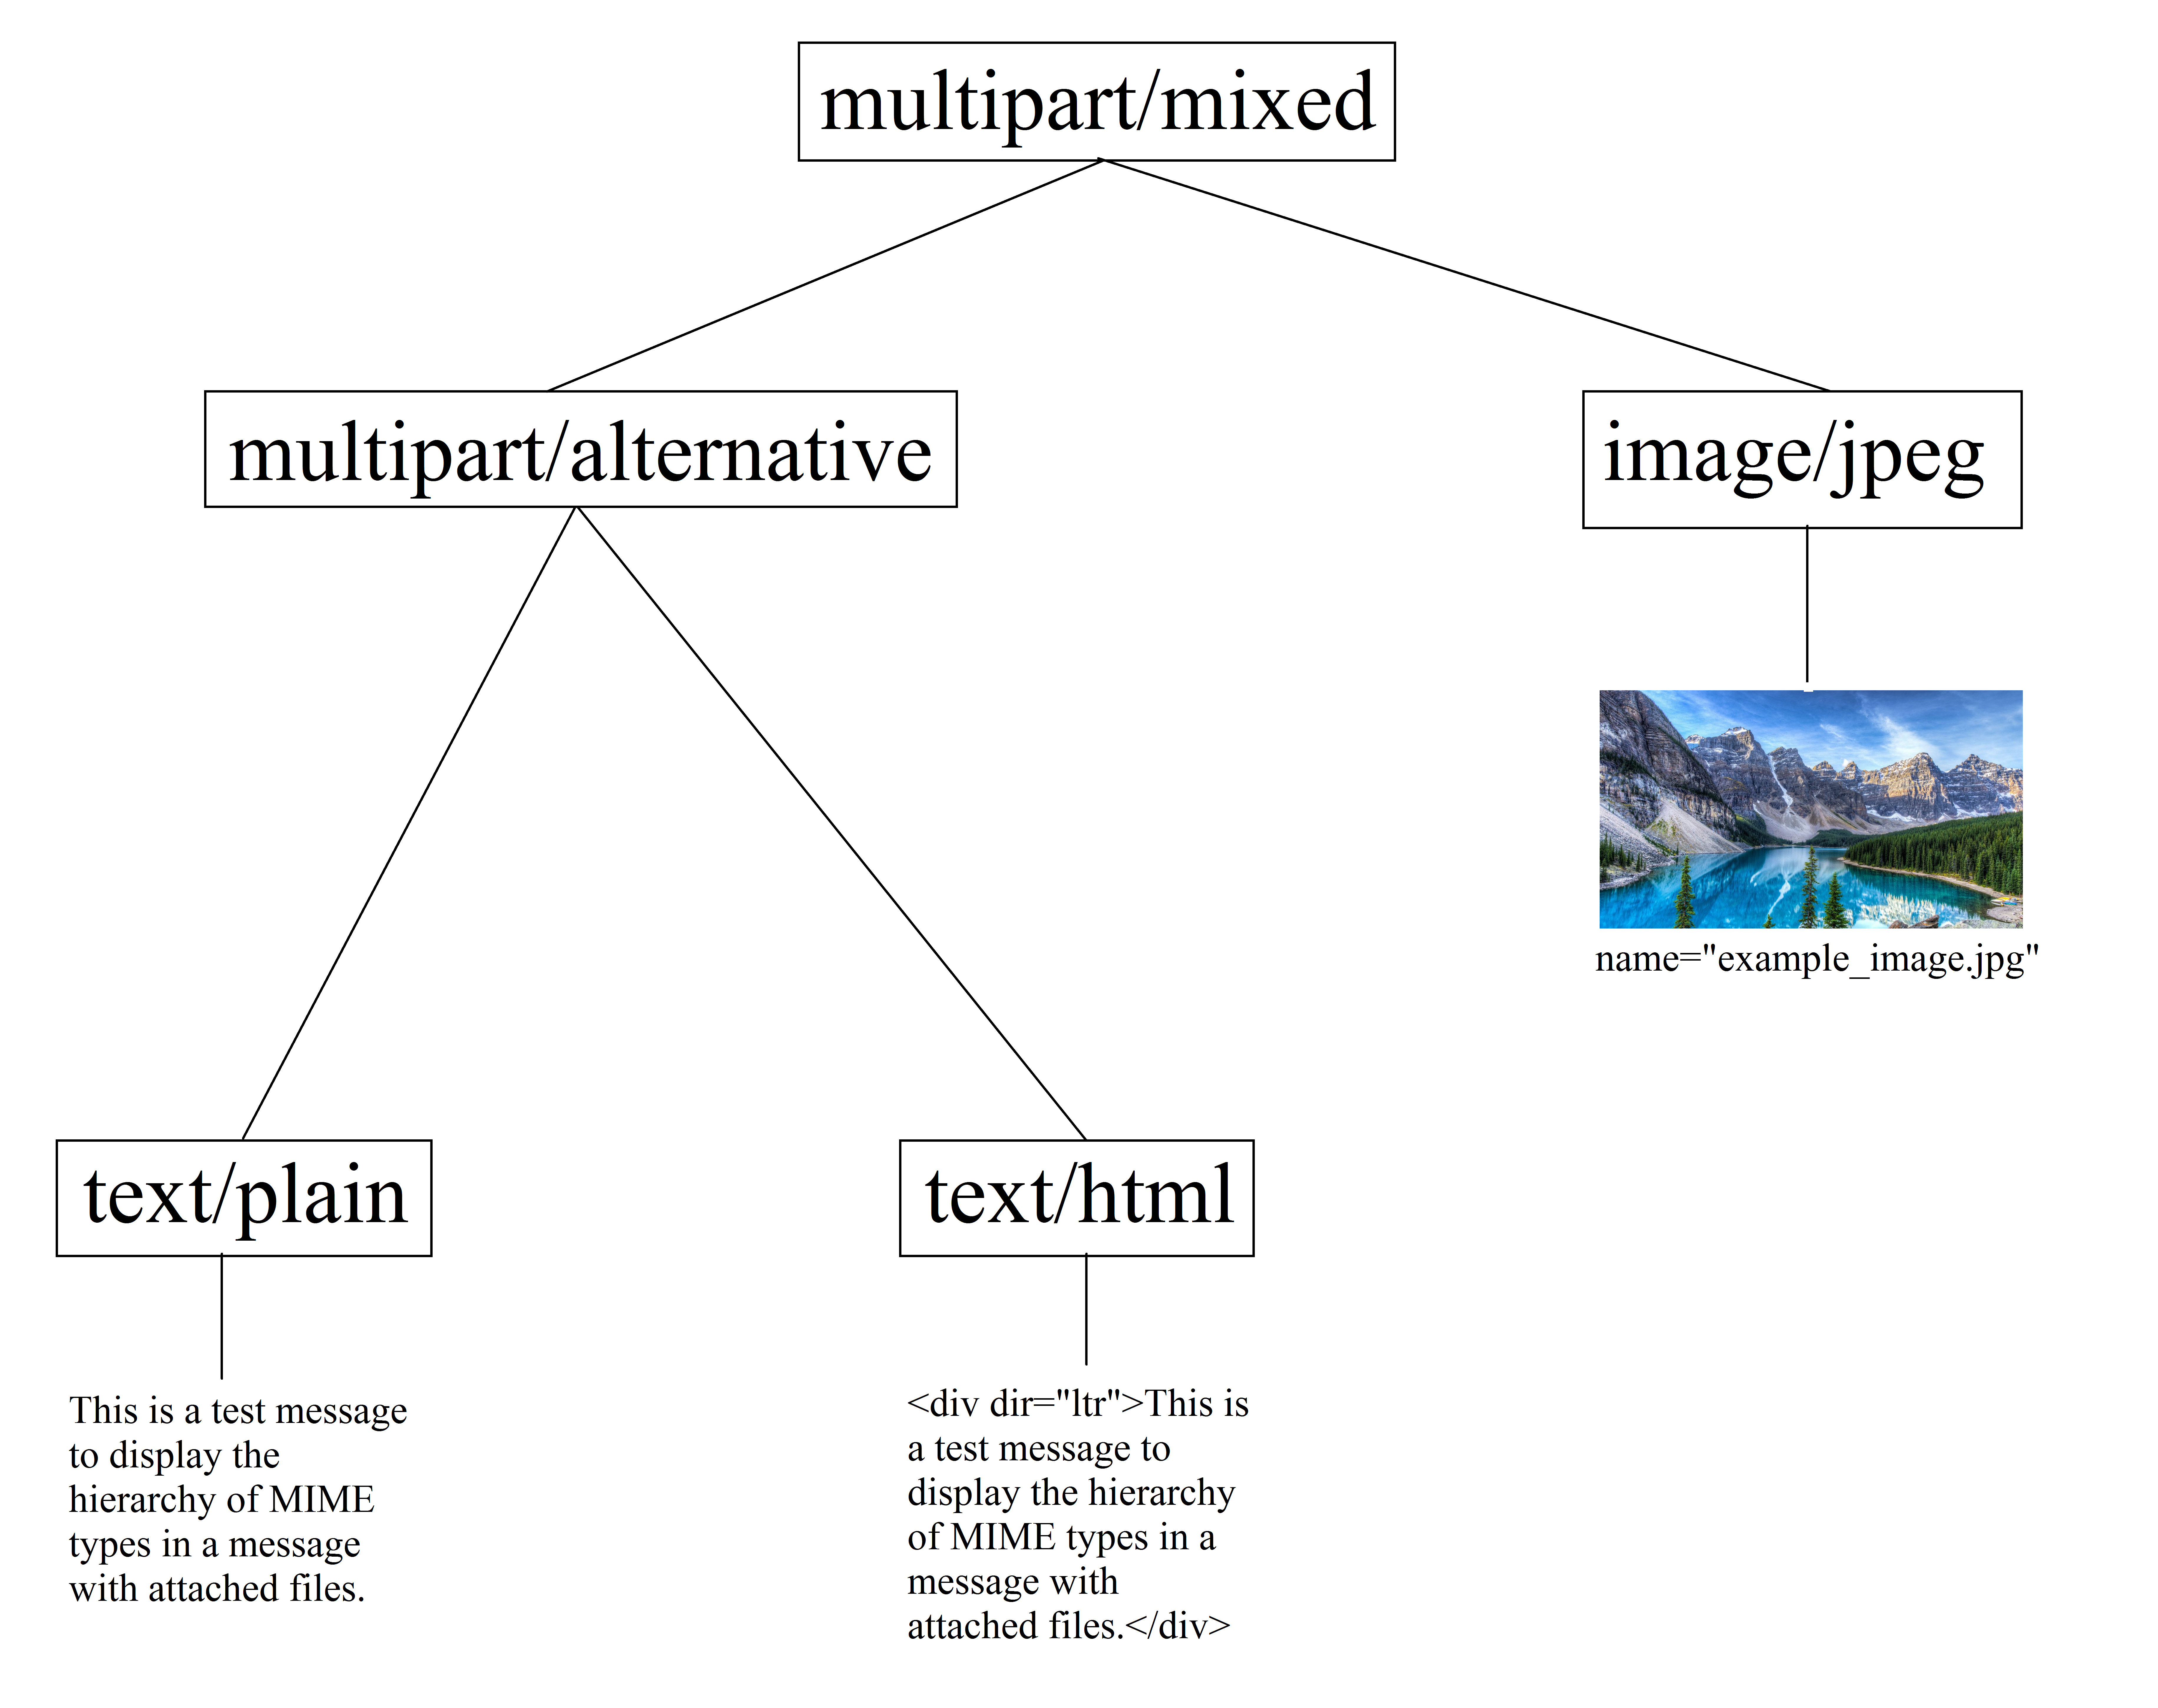
\includegraphics[width = 0.9\textwidth]{Imagenes/Bitmap/tree-content-type.png}}%
		\caption{Estructura arbórea de tipos MIME de un e-mail de ejemplo}%
		\label{fig:content-type}
		Imagen extraída de \cite{mitfg}
	\end{figure}

	\item\textit{Content-Disposition}: esta cabecera indica la forma de presentación de la parte del mensaje a la que pertenece. Puede tener dos posibles valores: \textit{inline} (que se utiliza cuando el contenido debe ser mostrado al mismo tiempo que el cuerpo del mensaje, como por ejemplo cuando se inserta una imagen en el texto y no como archivo adjunto) y \textit{attachment} (este valor determinará que la parte del mensaje requerirá algún tipo de acción por parte del usuario para visualizar el contenido, como por ejemplo en el caso de adjuntar un archivo). Además, esta cabecera dispone de distintos campos que reflejan más información acerca del contenido, como puede ser el nombre del archivo y la fecha de creación o de modificación. A continuación se presenta un ejemplo extraído de \cite{rfc2183} de esta cabecera y los campos que pueden acompañarle:
	
	\begin{lstlisting}
		Content-Disposition: attachment; filename=genome.jpeg;
		modification-date="Wed, 12 Feb 1997 16:29:51 -0500";
	\end{lstlisting}
	
	También puede observarse esta cabecera en la última parte del mensaje de ejemplo dela figura \ref{fig:examplemime}.
	
	\begin{figure}[t]
		\centering%
		\centerline{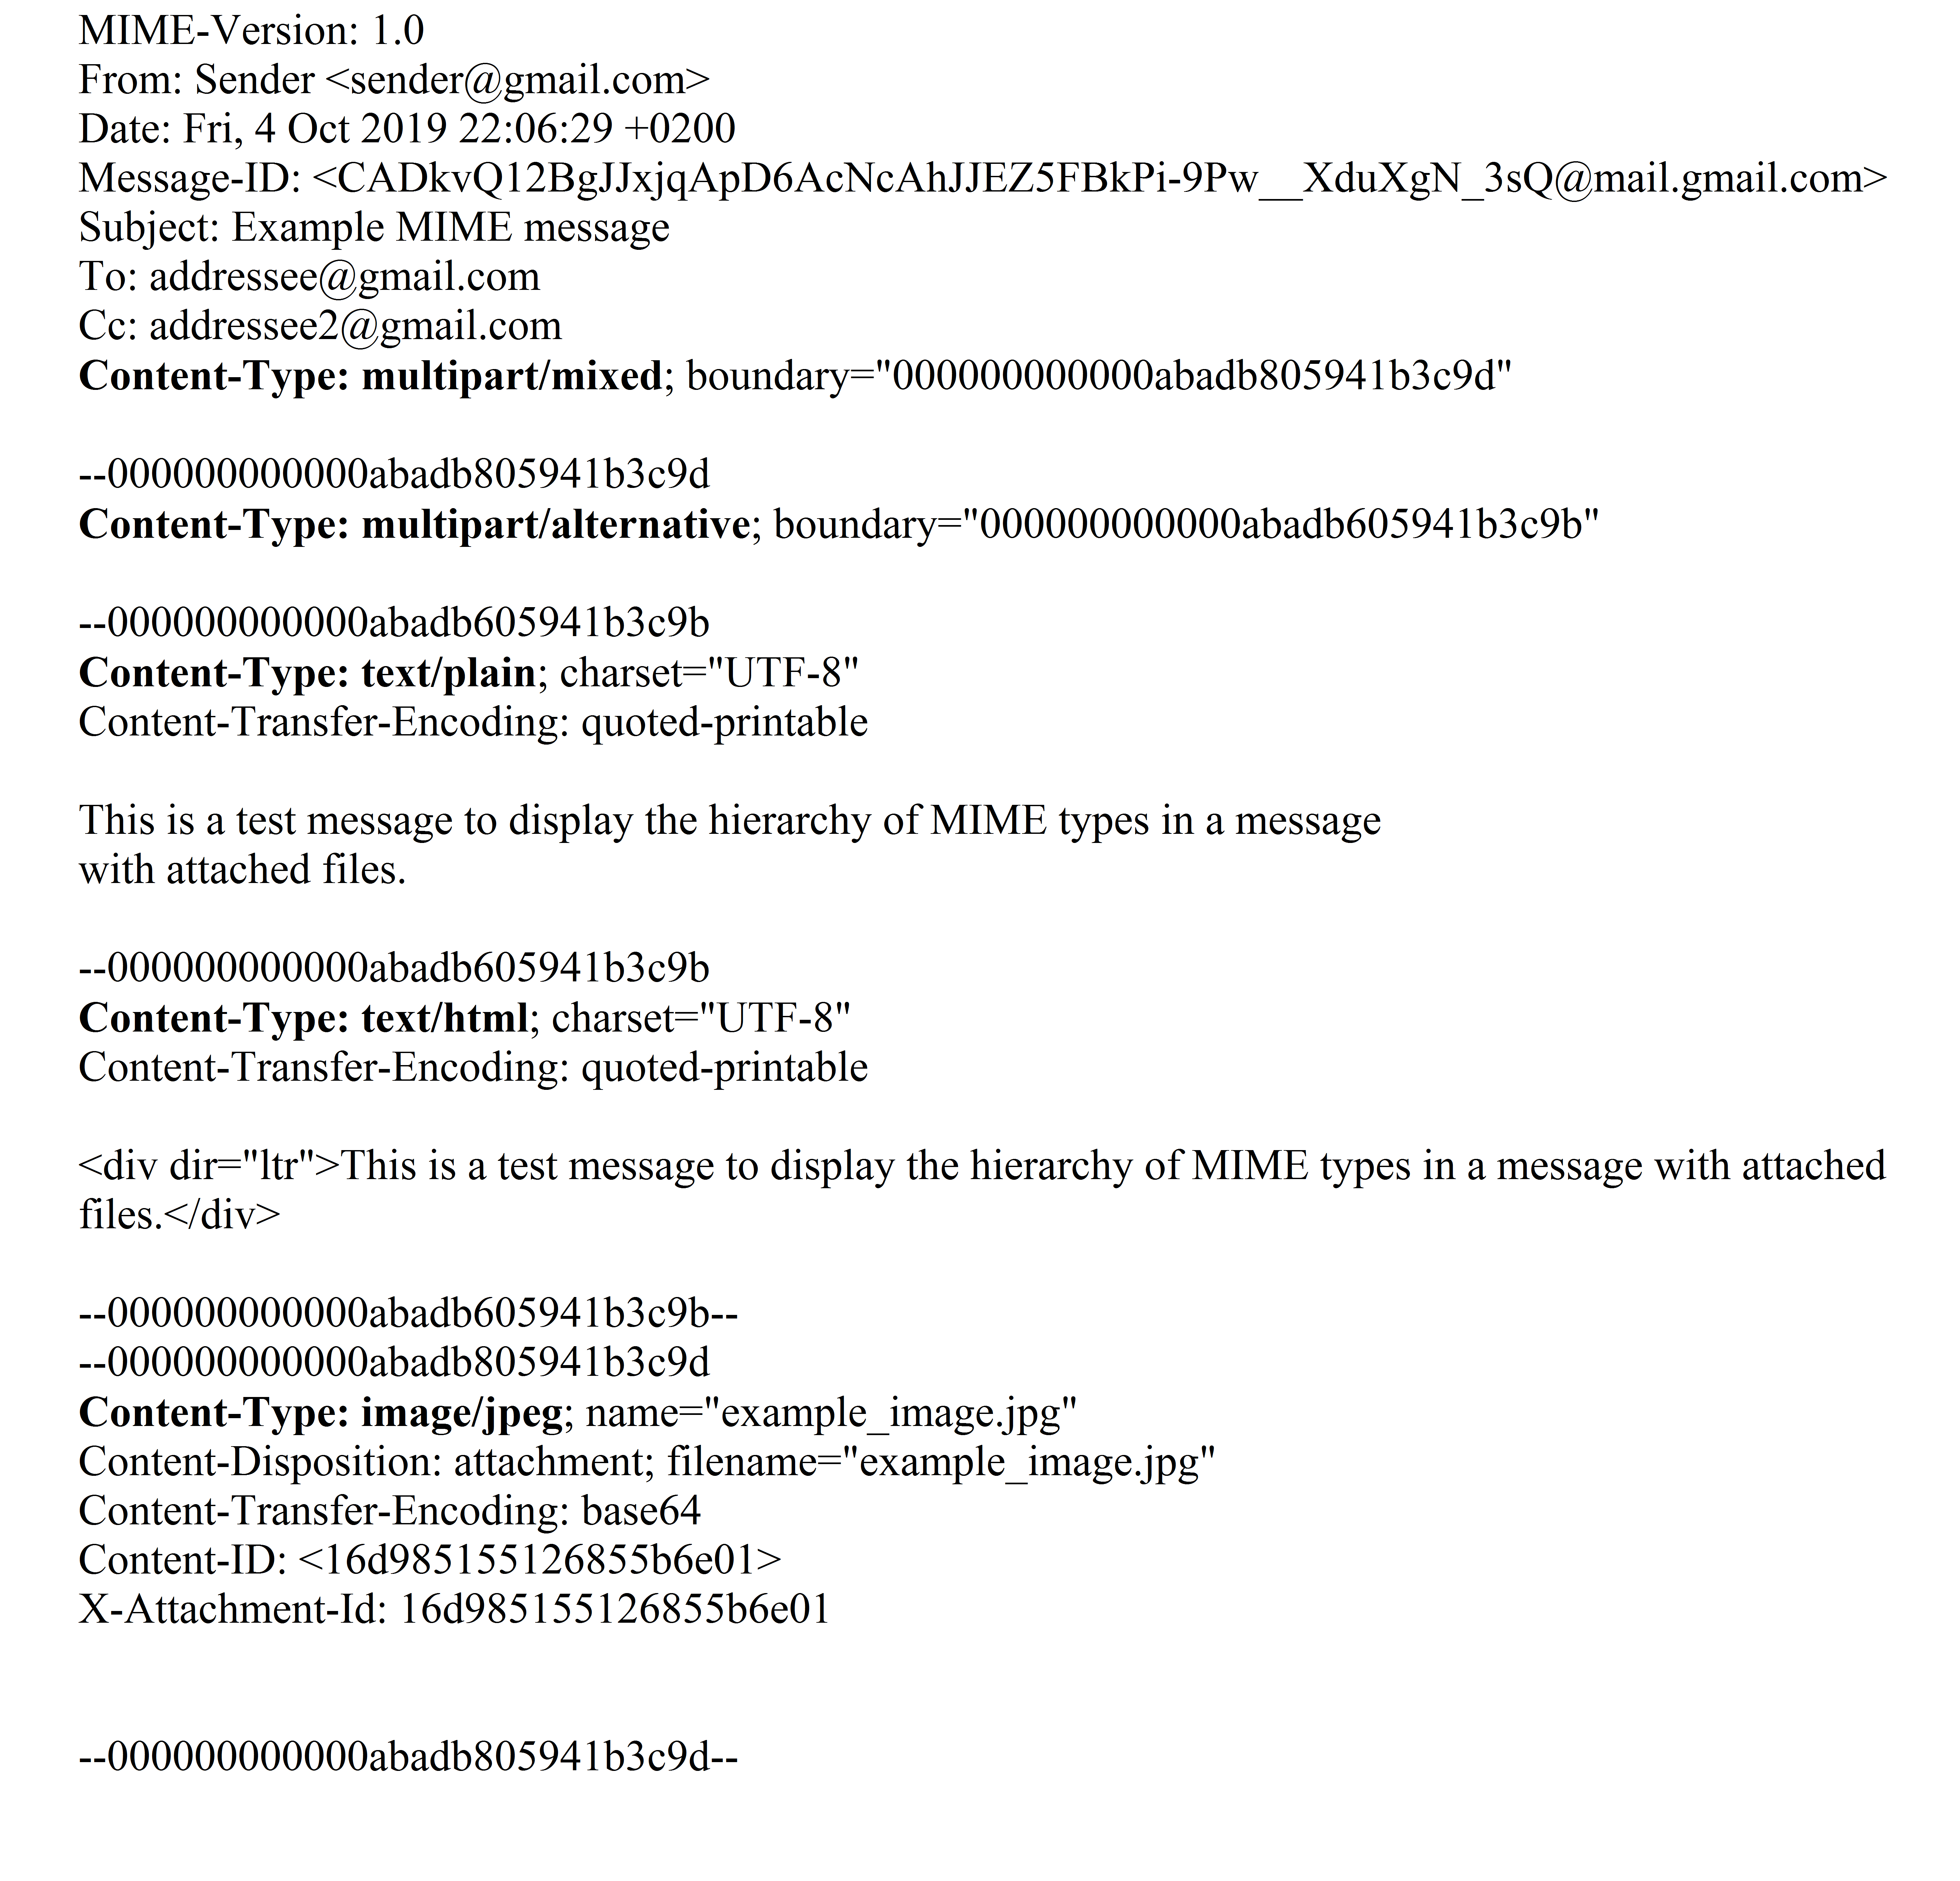
\includegraphics[width = 0.9\textwidth]{Imagenes/Bitmap/exampleMime.png}}%
		\caption{Mensaje MIME de la figura \ref{fig:content-type}}%
		\label{fig:examplemime}
		Imagen extraída de \cite{mitfg}
	\end{figure}
	\item\textit{Content-Transfer-Encoding}: cuando se mandan archivos en un correo electrónico, a veces estos se codifican como 8-bit o archivos binarios, codificaciones no soportadas por determinados protocolos. Por este motivo, es necesario poseer un estándar que especifique cómo debe re-codificarse este tipo de información en un formato 7-bit. La cabecera \textit{Content-Transfer-Encoding} \citep[Sección 5]{rfc1341} indica al cliente qué tipo de transformación se ha efectuado para que este sea capaz de recuperar los datos originales. Los posibles valores son \textit{base64} \citep{rfc4648, rfc2045}, \textit{quoted-printable} \citep{rfc1521}, \textit{8bit}, \textit{7bit}, \textit{binary} y \textit{x-token}. Todos ellos hacen referencia a un tipo de codificación que se encuentran fuera del alcance de este trabajo y para las que se recomienda consultar las referencias bibliográficas en caso de querer profundizar en ellas.
\end{itemize}

\subsection{SMTP}\label{ss:smtp}
El SMTP (cuyas siglas hacen referencia a \textit{Simple Mail Transfer Protocol}) es un protocolo de red orientado a conexión utilizado para el intercambio de correos electrónicos. Originalmente fue definido por \cite{rfc821} (para especificar cómo llevar a cabo el envío de mensajes) y \cite{rfc822} (que presenta el formato que deben tener los e-mails). Actualmente, se deben consultar los RFC desarrollados por \cite{rfc5321} y \cite{rfc5322} que, respectivamente, sustituyen a los dos originales.

Al ser un protocolo de transferencia de mensajes, posee algunas limitaciones a la hora de recibir e-mails en el servidor de destino. Por ello, esta tarea se delega a otros protocolos como el POP (véase la sección \ref{ss:pop}) e IMAP (véase la sección \ref{ss:imap}), mientras que el SMTP se encarga única y exclusivamente del envío.

Cuando se hace uso del SMTP un correo electrónico es enviado (esta acción de denota con la palabra \textit{push}) de un servidor a otro hasta que alcanza su destino. El mensaje se encamina en función del servidor de correo de destino, en lugar de hacerlo en función de los destinatarios individuales del mensaje especificados durante la conexión del cliente al servidor SMTP. Gracias a que este protocolo dispone de una función para iniciar el procesamiento de la cola de correo, un servidor de correo conectado de forma intermitente puede extraer mensajes de otro servidor remoto cuando sea necesario.

\subsection{POP}\label{ss:pop}
El POP (cuyas siglas hacen referencia a \textit{Post Office Protocol}) es un protocolo de aplicación en el modelo OSI utilizado para la obtención de e-mails almacenados en un servidor remoto de Internet denominado servidor POP. Originalmente fue definido por \cite{rfc918},que especificó la primera versión de POP, también conocida como POP1. La versión actual de POP, POP3 (en general cuando se habla de POP se refiere a esta versión), fue detallada por \cite{rfc1939}.

El protocolo POP posee numerosos comandos que hacen posible la conexión manual con el servidor POP3. Además, soporta otros como LIST, RETR y DELE, que permiten la gestión de los mensajes del usuario con acciones como mostrarlos, descargarlos o borrarlos, respectivamente.

POP3 fue diseñado para la tarea de recepción de correos electrónicos. Gracias a este protocolo, los usuarios con conexiones a Internet intermitentes o muy lentas pueden descargar sus mensajes mientras se encuentran conectados a la red y consultarlos estando \textit{offline}. La sucesión de operaciones más común se produce cuando un cliente se conecta, descarga todos sus mensajes, los almacena en su dispositivo local como e-mails nuevos, se borran del servidor y, por último, el usuario se desconecta. Sin embargo, algunos clientes de correo incluyen la opción de dejar los mensajes almacenados en el servidor en lugar de borrarlos. Estos utilizan el comando UIDL (\textit{Unique IDentification Listing}) el cual, a diferencia del resto de instrucciones de POP3, no identifica el correo electrónico a través del número ordinal asociado por el servidor, ya que generaría problemas si un cliente tratara de dejar ciertos mensajes en el servidor debido a que este número cambiaría de una conexión a otra. En lugar de ello, asigna a cada mensaje un identificador constituido por una cadena de caracteres única y permanente. De esta manera, se puede determinar fácilmente qué mensajes se quieren almacenar en el servidor a la vez que se descargan.

Al igual que otros protocolos más antiguos, POP3 utiliza un mecanismo de firma sin encriptación. De hecho, la transmisión de contraseñas POP3 en texto plano continúa ocurriendo. Hoy en día, POP3 tiene varios métodos de autenticación que ofrecen un amplio rango de niveles de protección contra accesos ilegales a las bandejas de correo de los usuarios.

La ventaja de POP3 frente a otros protocolos es que entre el cliente y el servidor no es necesario mandar un gran número de comandos para comunicarse. Este protocolo también resulta muy útil cuando no se cuenta con una conexión constante a Internet o a la red que aloja al servidor.

\subsection{IMAP}\label{ss:imap}
El IMAP (cuyas siglas hacen referencia a \textit{Internet Message Access Protocol}) es un protocolo de aplicación diseñado como alternativa al POP (véase la sección \ref{ss:pop}) en 1986, el cual permite el acceso a los mensajes almacenados en un servidor de Internet. Al igual que con el POP, con el IMAP es posible acceder a la cuenta de correo electrónico desde cualquier dispositivo con conexión a Internet. La versión actual del IMAP (IMAP versión 4 revisión 1 o IMAP4rev1) fue definida por \cite{rfc3501}.

A diferencia del POP, el IMAP abre la puerta a la gestión de la misma bandeja de entrada por parte de múltiples clientes. Esta característica se produce gracias a las principales diferencias entre los dos protocolos: el IMAP no elimina los mensajes del servidor hasta que el cliente lo solicite explícitamente (mientras que el POP los borra por defecto, lo que hace imposible acceder a ellos desde otro dispositivo que no haya descargado previamente los correos electrónicos) y tampoco descarga los e-mails en el dispositivo del usuario, aunque opcionalmente es factible tener una copia local de los mismos. Esta última propiedad del IMAP da lugar a algunas ventajas frente al POP. Una de ellas es la posibilidad e notificar de manera inmediata de la llegada de un nuevo correo electrónico (ya que el IMAP funciona con una conexión cliente-servidor permanente), mientras que el POP verifica si hay nuevos mensajes cada pocos minutos (lo cual provoca un aumento apreciable del tráfico y del tiempo que el usuario tiene que esperar para enviar una solicitud al servidor, ya que es necesario completar primero la descarga de todos los mensajes nuevos). Por otro lado, gracias al IMAP, los usuarios pueden crear carpetas compartidas con otras personas (esta funcionalidad depende del servidor de correo) y los e-mails no ocupan espacio de memoria en el dispositivo local, mientras que el POP los descarga independientemente de si van a ser leídos o no (estrictamente hablando, el IMAP tiene que descargar el mensaje cuando va a ser leído, pero se trata de archivos temporales y solo se extraen las cabeceras de los correos electrónicos a la hora de gestionar la bandeja de entrada). Precisamente, el hecho de evitar la descarga del e-mail, permite al usuario gestoinar carpetas, plantillas y borradores en el servidor además de poder llevar a cabo una búsqueda en la bandeja de entrada mediante palabras clave.

\section{Generación de Lenguaje Natural}\label{s:nlg}
%Intro de emails%
¿Y si fuera posible ahorrar todo este tiempo de escritura de correos electrónicos?

Para lograr este propósito es imprescindible profundizar en la rama de la Inteligencia Artificial conocida como \textit{Generación de Lenguaje Natural} (cuyas siglas son \textit{NLG} por su nombre en inglés \textit{Natural Language Generation}). Un buen ejemplo de aplicación de las técnicas de generación automática de textos son los 100.000 libros que Philip M. Parker puso a la venta en la plataforma \textit{Amazon.com} incluyendo títulos de temáticas tan variadas como \textit{El libro oficial del paciente sobre la estenosis espinal} \citep{parker2002official}, \textit{Perspectivas mundiales de 2009 a 2014 de los envases de 60 miligramos de Fromage Frais} \citep{parkerfromage},  \textit{Perspectivas de 2007 a 2012 de las tapetes de nudo, alfombras de baño y conjuntos que miden 6 pies por 9 pies o menos en la India} \citep{parkerrugs} y \textit{Tesauro Quechua - Inglés} \citep{parkerquechua}.

Resulta evidente que dicha cantidad de libros no pudieron ser escritos por Parker, sino que debió hacerse uso de técnicas de generación automática de textos. El algoritmo utilizado para dicho propósito, se engloba dentro de los métodos de generación conocidos como \textit{text-to-text} (texto a texto en castellano), dado que este tipo de técnicas toman como entrada textos ya existentes (normalmente escritos a mano y no generados automáticamente) y producen un nuevo texto coherente como salida. Otras aplicaciones de este tipo de métodos son la traducción automática de un idioma a otro \citep{hutchins2009introduction, oettinger2013automatic}, el resumen automático de textos \citep{mani2001automatic, nenkova2011automatic}, la simplificación de textos complejos, ya sea para hacerlos más accesibles para un público de lectores de bajo nivel de alfabetización \citep{siddharthan2014survey, bautista2011empirical} o niños \citep{macdonald2016summarising}, corrección automática de ortografía, gramática y texto \citep{kukich1992techniques, ng2014conll}, generación automática de revisiones de artículos científicos \citep{bartoli2016your}, generación de paráfrasis dada una frase de entrada \citep{bannard2005paraphrasing}, generación automática de preguntas con fines didácticos y educativos \citep{brown2005automatic}, generación automática de relatos dada una descripción conceptual de la historia deseada \citep{gervas2004story} o reescritura de textos (en concreto correos electrónicos) con estilo en función del destinatario \citep{mitfg}.

Además de estos métodos text-to-text, existen los llamados \textit{data-to-text} (datos a texto), en los cuales en lugar de recibir un texto como entrada, se genera el lenguaje a partir de datos. Estos pueden ser de todo tipo para dar lugar a informes o resúmenes como pueden ser de índole climatológica \citep{goldberg1994using, ramos2014linguistic}, financiera \citep{plachouras2016interacting}, ingenieril, como por ejemplo el trabajo desarrollado por \cite{yu2007choosing} para generar resúmenes de datos recopilados por sensores en turbinas de gas, sanitaria \citep{huske2003text, banaee2013towards}, como la investigación llevada a cabo por \cite{portet2009automatic} para obtener informes textuales a partir de datos de cuidados intensivos neonatales, o, incluso, deportivos \citep{theune2001data, chen2008learning}. Además de informes o resúmenes, también se utilizan los métodos \textit{data-to-text} para otros propósitos como la composición de discursos narrativos para relatos de varios personajes a partir de partidas de ajedrez \citep{gervas2014composing}, redacción de periódicos electrónicos a partir de datos de sensores \citep{molina2011generating}, generación de texto que aborda problemas medioambientales como el seguimiento de la fauna \citep{siddharthan2012blogging, ponnamperuma2013tag2blog}, la información medioambiental personalizada \citep{wanner2015getting} y la mejora del compromiso de los ciudadanos científicos a través de los comentarios generados \citep{van2016role} o producción de información interactiva sobre artefactos culturales \citep{stock2007adaptive}, entre otros.

Debido a que el objetivo de este trabajo se centra en la generación de correos electrónicos a partir del asunto, exploraremos en detalle las técnicas de Generación de Lenguaje Natural y, en especial, los métodos text-to-text. Para profundizar en los algoritmos y arquitecturas empleados ante los problemas de tipo data-to-text, conviene consultar la investigación llevada a cabo por \cite{gatt2018survey}, en la cual muestran el estado del arte de los trabajos realizados en este ámbito.

\subsection{¿Qué es la Generación de Lenguaje Natural?}
Dado que tanto los sistemas text-to-text como data-to-text y todas sus aplicaciones mencionadas anteriormente pertenecen a la rama de Generación de Lenguaje Natural, esta no debe definirse en función de la entrada del sistema, sino en la salida. Según \cite{biblia} la NLG es la conceptualización del ``campo de la inteligencia artificial y la lingüística computacional que se centra en los sistemas informáticos que son capaces de producir textos comprensibles en inglés u otra lengua humana. [...] Como área de investigación, la NLG presenta una perspectiva única ante problemas fundamentales de la inteligencia artificial, la ciencia cognitiva y la interacción. Estos incluyen cuestiones como por ejemplo cómo deben ser representados y cómo debe razonarse con la lingüística y el dominio del conocimiento, qué significa que un texto esté correctamente redactado y cómo es la mejor forma de comunicar información entre las computadoras y los usuarios.'' Por lo tanto, la Generación de Lenguaje Natural se puede definir como el ámbito que engloba el estudio de la producción de lenguaje no artificial, así como el diseño e implementación de algoritmos y sistemas computacionales cuyo resultado debe ser un texto que imite la forma en que los humanos se comunican verbalmente \citep{vicente2015generacion}, ya sea oralmente o por escrito \citep{del2007que}. Es decir, independientemente de la entrada recibida, se precisa el significado de NLG a partir de la salida esperada por el problema planteado. Tanto es así, que, como hemos visto, la entrada del sistema puede variar excesivamente \citep{mcdonald1993issues}: desde textos (que son precisamente los sistemas text-to-text) hasta datos de todo tipo como partidas de ajedrez \citep{gervas2014composing}, pictogramas \citep{gonzalez2019traductor} e, incluso, vídeos \citep{thomason2014integrating}. Sin embargo, autores como \cite{duvsek2020evaluating} acotan la definición de los sistemas de NLG estableciendo que la entrada deben ser representaciones semánticas, obviando así la primera tarea de la arquitectura propuesta por \cite{biblia} conocida como macro planificación o determinación del contenido (se explicará en la sección \textcolor{red}{poner nº}), que es precisamente el punto en el que se generan dichas representaciones semánticas.

Cabe destacar que, aunque desde un principio hayamos diferenciado entre métodos text-to-text y data-to-text, ni los límites entre las dos aproximaciones ni la pertenencia de algunas técnicas a ellas se encuentran claramente definidos. Un ejemplo de ello podemos encontrarlo en la generación automática de resúmenes de textos. En principio se caracterizaría claramente como un sistema text-to-text. No obstante, al hacer frente a este problema se han desarrollado soluciones con las conocidas técnicas abstractivas \citep{genest2011framework}, que, como explican \cite{hahn2000challenges}, a diferencia de los métodos de extracción evitan recoger las frases completas y se limitan a tomar unidades semánticas. Este tipo de técnicas usadas, por ejemplo, en la obtención de opiniones de reseñas para la posterior generación de frases nuevas \citep{labbe2012towards}, también provienen de problemas data-to-text. A la inversa, un sistema data-to-text puede hacer uso de técnicas que principalmente son utilizadas en los casos de uso text-to-text \citep{mcintyre2009learning, kondadadi2013statistical}. Por otro lado, podría parecer que los métodos de \textit{deep learning} \citep{goodfellow2016deep} deben ser mayoritariamente utilizados en los problemas data-to-text utilizando el trabajo llevado a cabo por \cite{mikolov2013efficient}. Sin embargo, se han desarrollado extensamente esta clase de soluciones para la NLG con gran variedad de arquitecturas como las redes neuronales recurrentes \citep{cho2014learning, tang2016context} muy a menudo combinadas con la memoria a corto plazo o LSTM \citep{chen2016enhanced}.

\chapter{Descripción del Trabajo}
\label{cap:descripcionTrabajo}

\chapterquote{¡Datos! ¡Datos! ¡Datos! - exclamó con impaciencia - No puedo hacer ladrillos sin arcilla}{El misterio de Copper Beeches\\Arthur Conan Doyle (1892)}

Aquí comienza la descripción del trabajo realizado. Se deben incluir tantos capítulos como sea necesario para describir de la manera más completa posible el trabajo que se ha llevado a cabo. Como muestra la figura, está todo por hacer.

Si te sirve de utilidad,  puedes incluir tablas para mostrar resultados, tal como se ve en la tabla.
\section{Tecnologías utilizadas}\label{s:tech}
Antes de comenzar con el desarrollo del trabajo realizado, en esta sección se introducen las distintas tecnologías que han sido empleadas para la implementación del proyecto. Debe tenerse en cuenta que la totalidad del trabajo ha sido desarrollado usando el lenguaje de programación Python, por lo que las herramientas que se presentan a continuación son compatibles con dicho lenguaje. 

Dado que el estudio gira en torno a los cuerpos de los correos electrónicos, es decir, se centra en el manejo de las cadenas de caracteres, es imprescindible un analizador sintáctico que facilite el análisis del corpus de partida. Para cubrir esta necesidad, se ha elegido spaCy, herramienta que se detalla en la sección \ref{ss:spacy}. Por otro lado, en lo relativo a las tareas relacionadas con el procesamiento de lenguaje natural, también se necesita poder obtener los Information Items dado un texto de entrada. Este problema puede implementarse gracias a la librería textaCy (véase el apartado \ref{ss:textacy}).

En cuanto al desarrollo de la arquitectura transformer, la cual consta de numerosas capas de redes neuronales, como se explicó en la sección \ref{sss:transformer}, será de gran ayuda la librería desarrollada por Google llamada Tensorflow (consúltese el apartado \ref{ss:tf}). Gracias a ella será posible presentar un modelo de aprendizaje automático que aborde todos los problemas de la generación de lenguaje natural.

Por último, se introduce el sistema de almacenamiento con el que se ha trabajado para contar con una gestión eficiente de los datos que se manejan: MongoDB (sección \ref{ss:mongodb}).

\subsection{spaCy}\label{ss:spacy}
Para ser capaces de llegar a conclusiones y estudiar el corpus de correos electrónicos seleccionado (véase la sección \ref{ss:enron}), se debe poder analizar el cuerpo de los mismos. Es decir, se necesita un analizador sintáctico que permita separar los diferentes textos en tokens (o dicho de otro modo, segmentar el texto en palabras, signos de puntuación, etcétera) y obtener diferentes características de ellos (como su categoría gramatical). Para conseguir ese objetivo, se va a utilizar la librería spaCy\footnote{\url{https://spacy.io/}}.

En esta sección se explican las razones por las que se elige spaCy (véase la sección \ref{ssect:spacywhy}) y su utilidad en el proyecto (véase la sección \ref{ssect:spacyut}).

\subsubsection{spaCy frente a otros analizadores sintácticos}\label{ssect:spacywhy}

Se ha elegido spaCy como analizador sintáctico frente a otros por varias razones, apoyadas por investigaciones publicadas como la realizada por \cite{choi2015depends}, y que se explican a continuación.

\begin{figure}[h]
	\centering%
	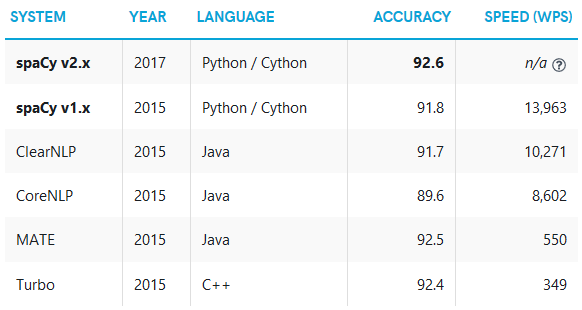
\includegraphics[width = 0.75\textwidth]{Imagenes/Bitmap/spacyeval.png}%
	\caption{Benchmarks de los distintos analizadores sintáctos}%
	Imagen extraída de \url{https://spacy.io/usage/facts-figures#benchmarks}
	\label{fig:spacyeval}
\end{figure}

Una evaluación publicada por \textit{Yahoo! Labs} y la Universidad Emory, como parte de un estudio de las tecnologías de análisis sintáctico actuales \citep{choi2015depends}, observó que ``spaCy es el analizador sintáctico voraz más rápido'' y su precisión está dentro del 1\% de los mejores existentes (como podemos ver en la figura \ref{fig:spacyeval}). Los pocos sistemas que son más precisos son, al menos, 20 veces más lentos. La velocidad es un factor importante cuando se quiere implementar sistemas complejos que se enfrentan a textos largos o a un gran número de documentos (como es el caso de este trabajo, en el que se quieren analizar todos los correos electrónicos posibles).

\begin{figure}[h]
	\centering%
	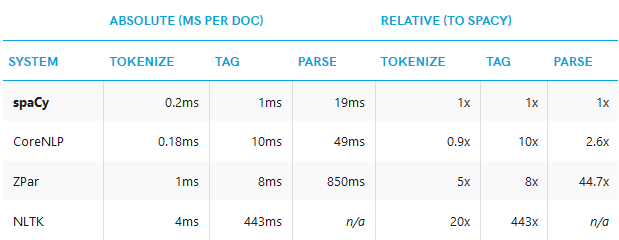
\includegraphics[width = 0.85\textwidth]{Imagenes/Bitmap/spacyspeed.png}%
	\caption{Tiempo de procesamiento por documento de varias librerías de NLP}%
	Imagen extraída de \url{https://spacy.io/usage/facts-figures#benchmarks}
	\label{fig:spacyspeed}
\end{figure}

Los resultados de \cite{choi2015depends} y las discusiones posteriores ayudaron a spaCy a desarrollar una novedosa técnica para mejorar la precisión del sistema, la cual fue publicada en un trabajo conjunto con la Universidad de Macquarie \citep{honnibal2015improved}. Por este motivo, se ha elegido una versión de spaCy que aprovecha esta técnica.

Además, no sólo en general, sino en cada tarea particular (tokenización, etiquetado y análisis sintáctico), spaCy es la más rápida si la comparamos con otras librerías de procesamiento del lenguaje natural. Esto se muestra en la figura \ref{fig:spacyspeed}, donde se puede observar tanto los tiempos absolutos (en milisegundos) como el rendimiento relativo (normalizado a spaCy). Los sistemas que tienen valores más bajos son más rápidos en sus tareas.

\subsubsection{Utilidades de spaCy}\label{ssect:spacyut}
Se puede definir spaCy como una biblioteca de procesamiento de lenguaje natural de Python diseñada específicamente para ser una biblioteca útil para implementar sistemas listos para la producción. Por esta razón, tiene una gran cantidad de utilidades diferentes. Sin embargo, sólo se necesitarán las que realizan el \textit{Tokenizer}.

La clase \textit{Tokenizer} de spaCy se encarga de dividir el mensaje dado en las diferentes palabras que lo constituyen y obtener varias características sobre ellas. Interesan los atributos que se pueden observar en la tabla \ref{tab:attspacy}. Además de su categoría gramatical, da más información (que no nos interesa) en función de su categoría léxica, como su género, número, tiempo verbal o, incluso, el tipo de adverbio.

\begin{table}[h]
	\begin{tabular}{|l|l|p{0.675\linewidth}|}
		\hline
		\textbf{Atributo} & \textbf{Tipo} & \textbf{Explicación}                                                                     \\ \hline
		is\_punct          & bool          & Indica si el token es un signo de puntuación \\ \hline
		is\_right\_punct   & bool          & Indica si el token es un signo de puntuación derecho (como el paréntesis cerrado). \\ \hline
		is\_left\_punct    & bool          & Indica si el token es un signo de puntuación izquierdo\\ \hline
		is\_bracket        & bool          & Indica si el token es un paréntesis\\ \hline
		like\_url          & bool          & Indica si el token es una url \\ \hline
		like\_email        & bool          & Indica si el token es una dirección de correo electrónico\\ \hline
		lema\_             & string        & Forma base del token sin sufijos o inflexiones\\ \hline
		is\_stop           & bool          & Indica si el token es una stop word\\ \hline
		pos\_              & string        & Categoría gramatical\\ \hline
		text & string & Verbatim text content. \\ \hline
		idx & integer & The character offset of the token within the parent document. \\ \hline
	\end{tabular}
	\caption{Atributos de interés de la clase \textit{Tokenizer}}\label{tab:attspacy}
\end{table}


\subsection{textaCy}\label{ss:textacy}

Sobre la librería de spaCy se han desarrollado múltiples soluciones para distintos problemas en el ámbito del procesamiento de lenguaje natural. Uno de estos proyectos es textaCy\footnote{\url{https://spacy.io/universe/project/textacy}}. Se trata de una librería que cuenta con la capacidad de extraer los Information Items (véase la sección \ref{ss:resumen}), definidos como tuplas sujeto-verbo-objeto, de un texto. Basta con añadir la tarea de extracción de los InIts al pipeline de spaCy y, cuando se procese un texto, se obtendrán de forma automática estas tuplas. De esta manera, se puede generar una entrada para los correos electrónicos del corpus (que serían la salida del sistema) con la que entrenar el modelo construido.

\subsection{Tensorflow}\label{ss:tf}
Mientras que spaCy y textaCy son herramientas fundamentales durante el análisis y procesamiento del corpus, la librería de código abierto Tensorflow \citep{abadi2016tensorflow} es la piedra angular del desarrollo de la arquitectura transformer implementada. Posee una amplia cantidad de funcionalidades para trabajar con tensores de manera eficiente, está especializada en los modelos de aprendizaje automático y permite ejecutar Keras utilizando Tensorflow como base, la cual es una librería especialmente diseñada para implementar arquitecturas de deep learning y que facilita la construcción, entrenamiento y evaluación de las mismas.

\subsection{MongoDB}\label{ss:mongodb}
Como se justificará más adelante en la sección \ref{ss:almacen}, se necesita almacenar una gran cantidad de correos electrónicos con el fin de poder trabajar de forma eficiente con ellos. Para esta tarea se ha elegido MongoDB que es un sistema de base de datos NoSQL de código abierto y orientado a documentos.

En lugar de almacenar los datos en tablas, como se hace en las bases de datos relacionales, MongoDB almacena estructuras de datos BSON (una especificación similar a JSON) con un esquema dinámico, lo que facilita y agiliza la integración de datos en determinadas aplicaciones \citep{gyHorodi2015comparative}. Además, no se requieren recursos potentes para trabajar con ella y, gracias a la flexibilidad que ofrece el ser una base de datos NoSQL, se puede realizar fácilmente modificaciones en el modelo conceptual de la base de datos sin tener que preocuparse por los cambios problemáticos entre claves primarias y foráneas entre tablas. Además, cuenta con drivers oficiales para el lenguaje de programación Python con el que se desarrolla la solución.

\section{Análisis de los datos}
El primer paso en todo trabajo de ciencia de datos e inteligencia artificial es el análisis de los datos con los que se cuenta para entrenar y probar el modelo. \textcolor{red}{Completar introducción}

\subsection{Enron corpus}\label{ss:enron}
Para llevar a cabo cualquier trabajo relacionado con la ciencia de datos e inteligencia artificial es necesario contar con un conjunto de datos con el que poder entrenar al modelo desarrollado. Cuando se trata de un estudio relacionado con la generación de lenguaje natural, el conjunto de datos se llama corpus y suele contener ejemplos de documentos reales redactados por humanos similares a los que se desea producir. En concreto, para este trabajo, se ha elegido el corpus conocido como Enron\footnote{\url{http://www-2.cs.cmu.edu/~enron/}}, dado que los correos electrónicos que contiene pertenecieron a la empresa con el mismo nombre. Precisamente se hicieron públicos tras una investigación legal llevada a cabo a esta compañía por parte de la Comisión Federal de Regulación de la Energía\footnote{\url{https://www.ferc.gov/}} de Estados Unidos.

Enron corpus contiene 517.401 correos electrónicos escritos en inglés de 150 usuarios distintos. Además de la ventaja de la gran cantidad de elementos pertenecientes a este dataset, también ha sido elegido por encontrar diversos trabajos sobre este mismo conjunto de e-mails, como el llevado a cabo por \cite{klimt2004introducing}.

Este corpus está organizado en una jerarquía de directorios (uno por cada usuario), en la que dentro de los principales se encuentran las correspondientes carpetas de la cuenta de correo electrónico del usuario en cuestión, como bandeja de entrada, enviados y directorios personalizados. En estas carpetas se encuentran, cada uno en un archivo separado, los distintos correos electrónicos del corpus. Un ejemplo de cómo se presentan los diferentes e-mails viene reflejado en la figura \ref{fig:emailenron}.

\begin{figure}[h]
	\centering%
	\centerline{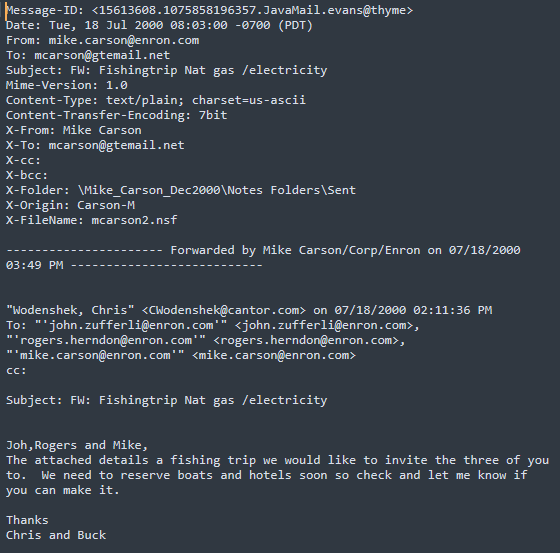
\includegraphics[width = 0.9\textwidth]{Imagenes/Bitmap/email-example.png}}%
	\caption{Ejemplo de un correo electrónico del corpus Enron}%
	\label{fig:emailenron}
\end{figure}

Como puede observarse en la figura \ref{fig:emailenron}, cada uno de los correos electrónicos se encuentra en un archivo distinto estructurado según el formato MIME explicado anteriormente (véase la sección \ref{ss:mime}). Claramente, se pueden diferenciar las distintas cabeceras de este formato con la información correspondiente a cada una de ellas. Después de todas estas cabeceras, se encuentra el cuerpo del mensaje. Por cada uno de los 517.401 correos electrónicos, se encuentra un archivo diferente con esta estructura.

\subsection{Preparación y limpieza de los datos}\label{ss:prep}

El primer problema que aparece ante el conjunto de datos elegidos es el formato en que se presentan cada uno de los correos electrónicos, ya que en cada archivo hay mucha información que generaría ruido y dificultaría el entrenamiento del modelo si no se eliminara (como las cabeceras MIME). Por ese motivo, es necesario preprocesar cada uno de ellos. Asimismo, se conseguiría un dataset apto para el propósito de construir un sistema de generación de lenguaje natural que redacte correos electrónicos.

Para extraer la información relevante de cada uno de ellos, el lenguaje de programación \textit{Python} cuenta con una librería\footnote{\url{https://docs.python.org/3/library/email.parser.html}} capaz de parsear correos electrónicos almacenados en archivos y cadenas de caracteres en formato MIME. Además, una vez procesadas las cadenas, la clase devuelta cuenta con una serie de métodos que facilitan la obtención de la información de las cabeceras y recorrer el árbol de partes MIME (véase la sección \ref{ss:mime} o consúltese el ejemplo de árbol representado en la figura \ref{fig:content-type}). De manera que solo ha sido necesario desarrollar un método que vaya recorriendo la estructura arbórea, comprobando el tipo MIME del nodo, y extrayendo el cuerpo del mensaje cuando lo encuentre.

Una vez se ha resuelto el problema de recuperar el correo electrónico dado el archivo perteneciente al corpus, es posible enfrentarse a otro reto antes del análisis exploratorio de los datos: la limpieza del cuerpo del mensaje para contar con un texto plano de cara al entrenamiento del modelo. Siempre, en todo trabajo en ciencia de datos, se presenta una fase de limpieza de los datos. Este paso resulta ligeramente más complicado cuando se está tratando con cadenas de caracteres. En el caso que ocupa a este trabajo, la limpieza consiste en encontrar patrones externos al cuerpo del mensaje, como la firma o la inclusión del mensaje al que se responde debajo de la respuesta, que no constituyen texto escrito por los usuarios, sino que ha sido incluido por el servidor de correo electrónico. Por ejemplo, en la figura \ref{fig:emailenron}, se muestra un e-mail el cual simplemente está reenviando otro mensaje distinto sin incluir más información. Esto resulta evidente por el comienzo del cuerpo del correo electrónico, que indica el reenvío. Este e-mail no debería incluirse en el entrenamiento de nuestro modelo, porque no añade información nueva y repite un mensaje que ya se tiene en otro archivo (dado que se cuenta con todos los correos del usuario, si el usuario está reenviando un e-mail, significa que es posible encontrar el mensaje original en la bandeja de entrada o alguna de las otras carpetas de su cuenta de correo). Por este motivo, es indispensable limpiar el cuerpo de los todos correos electrónicos del corpus.

Tras analizar concienzudamente el corpus de correos electrónicos se detectan varios patrones que deben abordarse y cambios que tienen que llevarse a cabo en los mensajes. El primero de ellos consiste en que, cuando un usuario contesta a un mensaje, el servidor incluye el mensaje que es respondido debajo de la contestación. En este caso solo interesa la respuesta y no el texto original (pues estará en otro archivo). No obstante, esta casuística no constituye un problema complicado de solventar, ya que se puede distinguir la respuesta del mensaje original porque siempre se incluye una cabecera de texto que no varía. Es decir, basta con encontrar la cabecera como subcadena en el cuerpo y eliminar todo lo que le preceda. La misma solución puede aplicarse al patrón que aparece cuando se envía un correo electrónico modificando una convocatoria de reunión. Resulta que el servidor genera una cabecera para diferenciar la modificación de la convocatoria original.

Ligeramente más complicado respecto a los patrones anteriores, aunque no demasiado, resulta el caso que se muestra en la figura \ref{fig:emailenron}. Se trata del reenvío de un e-mail. Cuando esto ocurre, la cabecera producida por el servidor no se trata de una subcadena fija, sino que incluye como información variable adicional el nombre del usuario que reenvía el correo, así como la fecha y hora en que se produce dicho reenvío. Aunque la solución sea la misma, eliminar lo que preceda a esta cabecera, no basta con buscar una subcadena que no varía, se requiere la utilización de expresiones regulares \citep{thompson1968programming}. Como la gran mayoría de lenguajes de programación, Python cuenta con un módulo para implementar expresiones regulares\footnote{\url{https://docs.python.org/3/library/re.html}} que ha facilitado enormemente esta tarea y ha hecho posible la limpieza de los mensajes con este patrón.

Otro problema que ha sido necesario abordar es el de la firma de los servidores de correo (frases al final de los mensajes como ``Get your FREE download of MSN Explorer''). Al ser siempre iguales, simplemente ha bastado con detectarlos y eliminar dicha subcadena del cuerpo de los mensajes. La dificultad de este tipo de limpieza de texto en realidad reside en detectar estos patrones, ya que, al tratarse de cadenas de caracteres, es complicado detectar incongruencias o errores.

Por último, debido al formato establecido por el protocolo MIME (por lo general depende de la codificación especificada para el mensaje), los servidores de correo electrónico incluyen tabulaciones y saltos de línea con una determinada frecuencia entre las palabras del texto, incluso aunque el usuario no los haya introducido. Dado que el salto de línea o la tabulación no es una información que se considere relevante de cara a la generación de texto de este modelo, se decide transformar estos caracteres en espacios y, a continuación, aplicar las expresiones regulares para detectar las subcadenas en las que se observe más de un espacio en blanco seguido y sustituirlas por uno solo.

Con esto concluye la limpieza de los cuerpos de los mensajes y la fase de preparación de los datos para adaptar los correos electrónicos a un formato adecuado para el sistema de almacenamiento elegido.

\subsection{Procesado y almacenamiento}\label{ss:almacen}

Como se ha explicado en el apartado \ref{ss:enron}, por defecto el corpus se almacena localmente estructurado en una jerarquía de directorios y contando con un archivo por cada correo electrónico. Sin embargo, esta forma de almacenamiento no resulta la más adecuada debido a que imposibilita cualquier método de búsqueda eficiente (sería necesario, en el peor de los casos, abrir todos los archivos para encontrar, por ejemplo, un e-mail en función del identificador del mensaje) y resulta excesivamente lento cuando se pretende procesar todos los mensajes (requiere recorrer la jerarquía como una estructura de datos arbórea entrando en todos los directorios). Por estas razones, la decisión de cambiar el sistema de almacenamiento es acertado para agilizar tanto la carga del corpus como las distintas operaciones que se pueden querer llevar a cabo sobre el mismo.

Como los elementos del conjunto son textos, es decir, datos no estructurados, un almacenamiento clásico en archivos de extensión \textit{.csv} podría provocar problemas como la elección del separador de los distintos campos, habría que utilizar un caracter que no apareciera en ningún cuerpo de mensaje ni en sus otras propiedades (asunto, identificador, destinatario, emisor, etcétera). Por lo tanto, un sistema relacional no parece que sea la mejor opción de almacenamiento para los correos electrónicos. Ante esta situación, se ha elegido el uso del sistema de base de datos NoSQL MongoDB (léase la sección \ref{ss:mongodb}) alojado en la nube\footnote{\url{www.mongodb.com/cloud}}. La decisión de no implantarlo en un repositorio local se sustenta sobre la ventaja que ofrece la nube de disponibilidad desde cualquier dispositivo, lo cual ha sido de gran ayuda en el proceso de desarrollo del trabajo.

Una vez se ha seleccionado la forma de almacenamiento, queda por determinar las colecciones que se van a crear y los campos de los que dispondrán los documentos. Una colección que es indispensable es la que albergará los correos electrónicos, la cual contará con la siguiente estructura:

\begin{python}
{
	# Identificador del documento mongo
	'_id' : ObjectId,
	# Identificador MIME del mensaje
	'Message-ID' : string,
	# Emisor del mensaje
	'From' : string,
	# Destinatario/s del mensaje
	'To' : string,
	# Asunto del mensaje
	'Subject' : string,
	# Cuerpo del mensaje
	'Body' : string,
	# Numero de palabras del cuerpo del mensaje
	'Number_of_Words' : integer,
	# Numero de Information Items del cuerpo del mensaje
	'Number_of_Inits' : integer
}
\end{python}

A excepción de los dos últimos campos, los demás se pueden extraer directamente mediante el uso de la librería específica de Python para mensajes en formato MIME (como se ha explicado en el apartado \ref{ss:prep}). Para obtener los dos últimos, es necesario procesar el cuerpo del mensaje antes de su almacenamiento en la nube. El primero, el número de palabras que contiene el cuerpo del correo electrónico, es posible hallarlo gracias al uso de spaCy (véase la sección \ref{ss:spacy}), librería que no solo tokeniza el texto, sino que nos permite distinguir entre los tokens que son palabras del resto, como, por ejemplo, signos de puntuación.

El último campo del documento que representa a los correos electrónicos, indica el número de Information Items (véase la sección \ref{ss:resumen}) que pueden extraerse del documento siguiendo la implementación llevada a cabo por \cite{genest2010text}. Estos InIts, que se definen como tuplas sujeto-verbo-objeto, se obtienen gracias a la librería textaCy (consúltese el apartado \ref{ss:textacy}), construida a partir de spaCy. De hecho, como se tratará en la sección \textcolor{red}{12345}, las representaciones semánticas abstractas que constituyen los Information Items serán la entrada de nuestro sistema de generación de lenguaje natural, por lo que, para evitar volver a extraerlos (su obtención es una operación computacionalmente costosa), será conveniente almacenarlos como otro documento de MongoDB. Dicha colección poseerá la siguiente estructura:

\begin{python}
	{
		# Identificador del documento mongo
		'_id' : ObjectId,
		# Identificador MIME del mensaje del que se extrajo el InIt
		'Message-ID' : string,
		# Sujeto del InIt
		'Subject' : string,
		# Verbo del InIt
		'Verb' : string,
		# Objeto del InIt
		'Object' : string
	}
\end{python}

Por ejemplo, si en el cuerpo del mensaje aparece la construcción lingüística ``I got change'' (en castellano ``tengo cambios''), se obtendrá el Information Item que se muestra en la figura \ref{fig:initexample}. De esta forma, es posible relacionar fácilmente un correo electrónico con sus InIts y viceversa.

\begin{figure}[h]
	\centering%
	\centerline{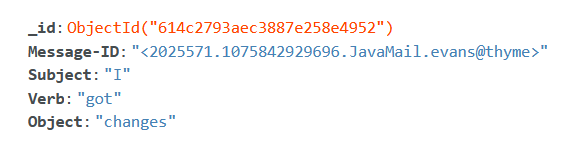
\includegraphics[width = 0.9\textwidth]{Imagenes/Bitmap/initexample.png}}%
	\caption{Ejemplo de documento de un Information Item}%
	\label{fig:initexample}
\end{figure}

Durante el proceso de almacenamiento, también se ha llevado a cabo un primer filtrado de mensajes que no son de utilidad para el propósito que persigue este trabajo y que, por tanto, pueden ser descartados sin guardarlos en MongoDB. Estos son: los correos electrónicos que carecen de cuerpo (puede ser porque originalmente no poseían o porque tras las operaciones de limpieza del mismo que han sido explicadas en la sección \ref{ss:prep}, se produzca esta situación), los e-mails de los que no se extrae ningún Information Item (ya que los InIts serán la entrada de nuestro sistema de generación de lenguaje natural) y los mensajes que son consecuencia de un error en el servidor de mensajería (por ejemplo, al intentar mandar un e-mail con una dirección de destinatario inexistente el servidor de correo siempre manda un mensaje informando de este error). De esta forma, se detectan 35.110 mensajes sin caracteres en el cuerpo, 121.799 correos electrónicos de los que no se extrae ningún Information Item y 7 e-mails consecuencia de errores en el servidor de mensajería, almacenando 360.485 correos electrónicos en la base de datos de MongoDB acompañados de 3.407.099 Information Items.

\subsection{Análisis exploratorio de los datos}\label{ss:eda}
Tras llevar a cabo las tareas de preparación, limpieza de los datos, procesamiento y almacenamiento, con un filtrado a priori, se pueden observar las distribuciones numéricas del corpus desarrollando un análisis exploratorio de los datos. Este estudio preliminar ofrecerá una descripción acerca de los correos electrónicos y sus Information Items.

El primer, y probablemente más sencillo, parámetro que puede analizarse es el número de palabras de cada correo. Para observar cómo se distribuye esta variable en el conjunto de datos, se han calculado las frecuencias requeridas para generar la figura \ref{fig:distpal}. En ella puede deducirse que, a pesar de poseer correos electrónicos con una gigantesca cantidad de palabras, la mayoría de mensajes muestran un número más considerable para tratarse de e-mails.

\begin{figure}[h]
	\centering%
	\centerline{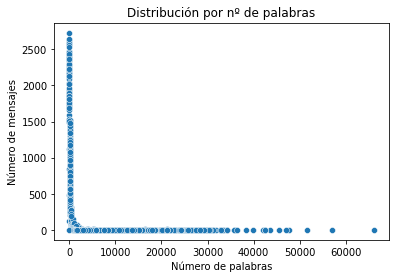
\includegraphics[width = 0.6\textwidth]{Imagenes/Bitmap/dist-palabras.png}}%
	\caption{Distribución del número de palabras en los mensajes}%
	\label{fig:distpal}
\end{figure}
\section{Implementación de una arquitectura realizer}\label{s:realizer}

El planteamiento inicial de este estudio era el de desarrollar una arquitectura realizer que fuera capaz de redactar correos electrónicos de manera automática. Como se explicó detalladamente en la sección \ref{sss:realizer}, el primer problema que surge ante esta propuesta son las estructuras de datos ad hoc generadas en función del dominio del que se quiere producir los textos de lenguaje natural. Esto resulta un inconveniente debido a que, a diferencia de aplicaciones con un dominio definido como pueden ser aquellas cuyo propósito es el de generar informes meteorológicos, la redacción automática de correos electrónicos resulta extremadamente difícil de enmarcar dentro de uno o varios dominios específicos. Además, el corpus que se ha elegido para entrenar el modelo, no se restringe a un tipo de temática de e-mails, sino que pueden encontrarse mensajes que versan sobre una gran variedad de temáticas. Esto complica más la implementación porque, aunque se limitara a un número razonable de asuntos y este hecho no fuera desvelado, el modelo podría ser capaz de aprender el lenguaje específico y las características lingüísticas inherentes a los dominios (por supuesto con mayor dificultad que si se fuera consciente de esta ventaja). Sin embargo, al no contar con esta facilidad, no existen entidades concretas o propiedades comunes más allá de las que posee el lenguaje general.

Si se estudia en detalle la arquitectura realizer, se observa que el mayor problema de restricción de dominio se encuentra en la fase de determinación del contenido. Por supuesto que en el resto de fases también está presente en mayor o menor medida, por ejemplo en la estructuración del documento, pero no posee tanta dependencia como esta primera tarea localizada en el pipeline de las arquitecturas de generación de lenguaje natural. La razón es que resulta sumamente complicado conceptualizar en una estructura de datos concreta, cualquier posible intención que se pueda tener a la hora de transmitir cualquier información. Aún así, la solución traída desde el ámbito del resumen abstractivo de textos, en la que dichas intenciones se materializan en tuplas sujeto-verbo-objeto, solucionaba en gran medida la dificultad del paso de determinación de contenido. Es decir, esta fase se resolvía mediante la generación de Information Items que indican los temas que se desean tratar a lo largo de todo el correo electrónico. De hecho, la gran ventaja de llevar a cabo esta aproximación es que, no solo abordaba el problema de determinación del contenido que, en principio, parecía insalvable, sino que también ofrecía una solución para generar la entrada para el entrenamiento del sistema. Dicho de otro modo, el corpus elegido no proporciona más que los correos electrónicos, que en teoría son la salida final del sistema de generación de lenguaje natural, por lo que no se cuenta con una entrada. Con la solución de las tuplas sujeto-verbo-objeto, es posible conseguir una supuesta entrada desde la que podrían haberse redactado los mensajes. Esto da paso a la utilización de técnicas de aprendizaje supervisado y evita tener que producir una entrada escrita a mano. En resumidas cuentas, con los Information Items ``matábamos dos pájaros de un tiro'': se conseguía un método de generación automática de una entrada para los correos electrónicos ya generados y se solventaba el problema de no ser capaces de concretar el dominio de los e-mails del corpus de cara a diseñar estructuras de datos ad hoc necesarias para implementar la fase de determinación del contenido. Sin embargo, los Information Items introducen un problema sumamente complicado de abordar. Al tratarse de estructuras genéricas que pueden versar sobre cualquier temática, esto impide que puedan usarse técnicas que añadan algún tipo de información adicional en la generación del texto. El origen de este gran escollo es que las fases subsiguientes a la determinación de contenido son altamente dependientes de la salida de esta última. Cuando el dominio es concreto se puede razonar sobre el contenido (con técnicas como las ontologías) o contar con entidades preestablecidas para añadir información extra al texto producido, mientras que al no poder enmarcarse dentro de uno o varios dominios, actualmente no existe la forma de razonar sobre conocimiento general. En consecuencia, el sistema de generación de lenguaje natural se limitaría a recibir las tuplas sujeto-verbo-objeto y construir estructuras lingüísticas que incluyeran única y exclusivamente la información semántica que transmiten los InIts en cuestión. Es decir, simplemente se podrían producir, a lo sumo, tantas oraciones como Information Items se recibiera y la única tarea sería la de generar las escasas estructuras sintácticas que faltaran, así como ajustar algunas categorías morfológicas como el tiempo de los verbos y el género y número de las palabras. Esta técnica de Information Items solo ha sido empleada en los sistemas de resumen automático de textos, precisamente porque impide que en el resto de fases se pueda añadir información adicional más allá de estructuras sintácticas necesarias para la correcta construcción de las oraciones.

Ante este panorama en que las fases subsiguientes a la determinación de contenido poseen una dependencia excesivamente alta cuando se utilizan los Information Items, se descartó la posibilidad de desarrollar este sistema siguiendo el esquema de arquitectura realizer y se optó por generar la aplicación siguiendo el modelo transformer.
\section{Implementación de la arquitectura transformer}\label{s:transformer}

A diferencia de los problemas que se encuentran al tratar de construir una arquitectura realizer para un problema sin dominio específico como es la redacción automática de correos electrónicos, los transformers son capaces de afrontar la generación de lenguaje natural sin la necesidad de enmarcar los textos dentro de un ámbito concreto. De hecho, normalmente se suele acudir a esta arquitectura cuando se pretende hacer frente a problemas en los que podría requerirse un conocimiento general.

Como en el apartado \ref{sss:transformer}, se entró bastante en detalle en la estructura de la arquitectura, cada uno de sus módulos y la filosofía detrás de cada uno de ellos, esta sección se limitará a exponer las vicisitudes específicas del problema que compete a este trabajo, empezando por la entrada de la aplicación.

La entrada del modelo debe ser un conjunto de no más de seis Information Items construidos como tuplas sujeto-verbo-objeto. Sin embargo, esto no coincide del todo con la definición de la entrada del modelo transformer. Para resolverlo, en primer lugar se tomará la lista de todos los InIts y se tokenizarán por separado. La tarea de tokenización se lleva a cabo utilizando un tokenizador preentrenado\footnote{\url{https://www.tensorflow.org/text/api_docs/python/text/BertTokenizer}}.

Con una lista de las tuplas Inits tokenizadas, se concatenan como si constituyeran un solo tensor. Esto podría generar la preocupación de que es necesario antes homogeneizar los tensores asegurándose de que todos los sujetos poseen la misma longitud mediante la técnica de \textit{padding} (todos los tensores se adaptan a la longitud del mayor de ellos rellenando con ceros las últimas dimensiones), y lo mismo con los verbos y objetos. No obstante, además de ser una operación computacionalmente costosa, no es necesario para el correcto funcionamiento de nuestro modelo. El motivo por el que se pueden concatenar los InIts (sobra decir que siempre todos ellos deben seguir el orden sujeto-verbo-objeto, ya que esto sí podría dificultar el entrenamiento y confundir al modelo) y luego hacer padding es que, como se explicó en la sección \ref{sss:transformer}, existen tokens especiales de inicio y fin. Estos se añaden a cada sujeto, verbo y objeto por separado, quedando así todos los elementos claramente delimitados. Es decir, la red neuronal aprenderá a distinguir dónde acaba un elemento de la tupla InIt y dónde comienza el siguiente sin necesidad de incluir ceros entre ellos. Este hecho, no solo ahorra tiempo computacionalmente hablando, sino que también ahorra en memoria, pues los vectores tokenizados de InIts son notablemente más pequeños, y, al reducir el tamaño de los vectores de Information Items, disminuye la entrada de la red y, por ende, el número de parámetros a entrenar.

Tras construir la tokenización de los Information Items, se tokeniza, con el mismo tokenizador preentrenado, el correo electrónico ``resultante''. Así ya se cuenta con la entrada, el tensor concatenado de InIts, y la salida de la red, el tensor del cuerpo del mensaje tokenizado. De esta manera, se está en disposición de entrenar el modelo y evaluar los resultados obtenidos.
%\include{Capitulos/Capitulo4}
%\include{Capitulos/Capitulo5}
\chapter{Conclusiones y Trabajo Futuro}
\label{cap:conclusiones}

\chapterquote{Difícil de ver es. Siempre en movimiento el futuro está}{Yoda - Star Wars: Episodio III - La venganza de los Sith (2005)}

Tras el desarrollo de este trabajo, en este capítulo se presentan las conclusiones que pueden extraerse de este estudio (se explican en la sección \ref{s:concl}). Justo después, las posibles opciones para la continuación de este trabajo quedan expuestas en la sección \ref{s:fut}, con el fin de continuar con el estudio de la generación de lenguaje natural a partir de representaciones semánticas.

\section{Conclusiones}\label{s:concl}

Hoy en día, el correo electrónico es un sistema de comunicación que se utiliza tanto en el ámbito profesional como en el personal. A través de él se establecen conversaciones sobre el trabajo, los estudios, relaciones íntimas, etcétera. Sin embargo, el gran número de e-mails que se reciben y envían cada día, comienza a obligar a sus usuarios a dedicar una notable cantidad de tiempo a atender su bandeja de entrada y pensar cuál es la mejor forma de redactar los mensajes, para transmitir la idea que se tiene en mente. Pero, ¿y si se pudiera escribir de forma automática con tan solo introducir como entrada dicha idea o concepto sobre el que giraría el cuerpo del mensaje? Este problema puede ser resuelto mediante el uso de técnicas de generación de lenguaje natural, un campo de la inteligencia artificial que se enfrenta al reto de producir textos imitando la forma en que los humanos se comunican entre sí. Dentro de esta rama, destacan dos tipos de arquitecturas: los modelos realizer y los modelos transformer. La primera aproximación consiste en un pipeline de tareas que, poco a poco, construyen el texto de salida; mientras que la segunda hace uso de los modelos de atención y las arquitecturas codificador-decodificador de deep learning. En este trabajo se trata de evaluar la viabilidad de implementar cada una de ellas para enfrentarse al problema de redacción automática de correos electrónicos, desarrollar la solución y valorar los resultados obtenidos.

Para representar esa idea que el usuario posee, se hace uso de los llamados Information Items, entidades que almacenan la mínima información semántica. Este elemento proviene de la rama del resumen automático de textos. Los Information Items serán la entrada del sistema desarrollado, representando ese concepto que posee el usuario acerca de lo que quiere redactar en el correo electrónico. Concretamente, se implementan mediante tuplas sujeto-verbo-objeto. Sin embargo, como se ha mostrado en el trabajo, esta definición no funciona adecuadamente en ninguna de las dos arquitecturas, ya que obliga al sistema de generación de lenguaje natural a producir construcciones lingüísticas con elementos semánticos no transmitidos por el usuario y que no puede obtener de otra manera.

En lo que se refiere al modelo realizer, las tuplas sujeto-verbo-objeto, solventan el problema de construcción de estructuras ad hoc para hacer frente a la fase de determinación del contenido, es decir, permiten implementar dicha tarea a pesar de que los correos electrónicos no se enmarquen en uno o varios dominios específico. No obstante, como en esta arquitectura el resto de fases poseen una alta dependencia de la salida de la determinación del contenido, que serían los Information Items, el texto producido se restringe a cada uno de ellos sin poder aportar más información semántica. Esto se debe a que no se cuenta con una base de conocimiento o módulo de razonamiento general de los que sacar dicha información extra que se pueda añadir al texto producido.

Respecto al modelo transformer, podría ocurrir que se añadiera información extra que aumentara el tamaño y la riqueza del cuerpo del correo electrónico. Sin embargo, al no poseer más contexto que los Information Items, si se incluyera, se trataría de estructuras lingüísticas basadas en la frecuencia de aparición del resto de correos electrónicos. Esto, limita enormemente la salida del sistema, así que requiere una inmensa cantidad de documentos en el corpus, mayor de la que se tiene, para poder producir el texto como esperaría el usuario final. Todas estas razones justifican los resultados obtenidos con dicha arquitectura y demuestran que la aproximación con esta definición de las representaciones semánticas que constituyen los Information Items, no permite alcanzar una generación de lenguaje natural de buena calidad, coherencia y cohesión.

\section{Trabajo futuro}\label{s:fut}
En vista de los resultados obtenidos, la principal vía de trabajo futuro es el estudio de la redacción automática de correos electrónicos utilizando otras implementaciones más complejas de los Information Items. La clave reside en que almacenen la suficiente información como para ser capaces de generar por completo el mensaje, pero no excesiva como para que el usuario tenga que redactar prácticamente todo el texto. Varias alternativas se han propuesta en el capítulo \ref{cap:estadoDeLaCuestion}, que pueden ser estudiadas individualmente o en conjunto. Por ejemplo, sería posible combinar el etiquetado del rol semántico con técnicas de desambiguación del sentido de las palabras.

No obstante, no se debe descartar la posibilidad de que quizás, con un mayor conjunto de entrenamiento, la propuesta desarrollada a lo largo de este trabajo obtenga resultados satisfactorios. Por esa razón, otra opción para continuar el trabajo desarrollado es la reutilización de los módulos implementados (que pueden encontrarse en el repositorio correspondiente\footnote{\url{https://github.com/carlosmmorera/NLG-AI-Master-Thesis}}) y entrenarlos con un corpus mayor que permite exprimir la utilidad de los InIts.

Por otro lado, es posible estudiar mejoras de cara a la arquitectura realizer con las que quizás, se podrían obtener resultados más satisfactorios. Estas mejoras van desde la reformulación de los métodos de redacción de pequeñas partes del mensaje, como la implementación de un modelo probabilístico para la generación automática del saludo en los correos electrónicos, hasta el desarrollo de un sistema de razonamiento con el que deducir otros Information Items e incluirlos al cuerpo del mensaje.

En cuanto a trabajo futuro en la arquitectura transformer, es razonable pensar que la división del problema de redacción en distintas partes, como lo que se ha propuesto antes de redactar fragmentos del e-mail, pueda concluir en resultados más satisfactorios. Además, también podría estudiarse la posibilidad de incluir más información de entrada, como los metadatos del correo electrónico (destinatario, asunto, etcétera) para extraer de ellos información extra que se pueda incluir en la redacción.

Estas son algunas vías posibles de trabajo futuro, de cara al estudio del caso de uso de redacción automática de correos electrónicos utilizando técnicas avanzadas de inteligencia artificial y, en concreto, del campo de la generación de lenguaje natural.

%%%%%%%%%%%%%%%%%%%%%%%%%%%%%%%%%%%%%%%%%%%%%%%%%%%%%%%%%%%%%%%%%%%%%%%%%%%
% Si el TFM se escribe en inglés, comentar las siguientes líneas 
% porque no es necesario incluir nuevamente las Conclusiones en inglés
%\begin{otherlanguage}{english}
%\chapter{Introduction}
\label{cap:introduction}

Introduction to the subject area. This chapter contains the translation of Chapter \ref{cap:introduccion}.

\section{Motivation}
The recent development and consequent growth that smartphones have brought about overthe last few decades has brought with it innumerable paradigm alterations, both in terms oftechnology and in the social sphere. Precisely, the easy and increasingly simple access thatcame with the appearance of smartphones connected to a 3G network in the early 2000s brought tools, nowadays considered essential, such as videoconferencing or instant messaging, to an emerging and growing public. It was precisely this ``pioneer'' messaging system that ended up evolving and leading to the development of different applications that have helped to popularize real-time communication, with up to 100 billion messages being sent daily by 2020. Although this series of applications have the main characteristic of being closer, more informal and immediate -so that the need for immediacy and the urgency of the addressers. Although it is true that, nowadays, e-mail is generally and usually intended for more formal or institutional environments, as a prelude to a communication that will probably evolve towards other types of platforms or, more informally, for sending files, it continues to be a means of communication in regular use; in the case of some people, this use even extends to the daily environment, but with the clear and obvious disadvantage that it requires greater attention from the user.

It is obvious that there is a significant gap between instant messaging applications and e-mail and that this gap must be overcome in order to facilitate the experience and use of e-mail for its users; therefore, IRIS is proposed. The IRIS (Intelligent Response Instantly Sent) system is proposed as a virtual assistant whose objective is to improve the user experience in the use of e-mail, addressing the problem of the required dedication that it demands; therefore, the modus operandi of IRIS is simple. When using IRIS, the user postulates the idea they want to convey and the subject around which the body of the message should revolve and this is received by the assistant, which, by using natural language generation techniques, will try to express this idea in a text format in an extensive manner, to subsequently send the e-mail to its addressee.










%\chapter{Conclusions and Future Work}
\label{cap:conclusions}

Conclusions and future lines of work. This chapter contains the translation of Chapter \ref{cap:conclusiones}.



%\end{otherlanguage}
%%%%%%%%%%%%%%%%%%%%%%%%%%%%%%%%%%%%%%%%%%%%%%%%%%%%%%%%%%%%%%%%%%%%%%%%%%%

%
% Bibliografía
%
% Si el TFM se escribe en inglés, editar TeXiS/TeXiS_bib para cambiar el
% estilo de las referencias
%---------------------------------------------------------------------
%
%                      configBibliografia.tex
%
%---------------------------------------------------------------------
%
% bibliografia.tex
% Copyright 2009 Marco Antonio Gomez-Martin, Pedro Pablo Gomez-Martin
%
% This file belongs to the TeXiS manual, a LaTeX template for writting
% Thesis and other documents. The complete last TeXiS package can
% be obtained from http://gaia.fdi.ucm.es/projects/texis/
%
% Although the TeXiS template itself is distributed under the 
% conditions of the LaTeX Project Public License
% (http://www.latex-project.org/lppl.txt), the manual content
% uses the CC-BY-SA license that stays that you are free:
%
%    - to share & to copy, distribute and transmit the work
%    - to remix and to adapt the work
%
% under the following conditions:
%
%    - Attribution: you must attribute the work in the manner
%      specified by the author or licensor (but not in any way that
%      suggests that they endorse you or your use of the work).
%    - Share Alike: if you alter, transform, or build upon this
%      work, you may distribute the resulting work only under the
%      same, similar or a compatible license.
%
% The complete license is available in
% http://creativecommons.org/licenses/by-sa/3.0/legalcode
%
%---------------------------------------------------------------------
%
% Fichero  que  configura  los  parámetros  de  la  generación  de  la
% bibliografía.  Existen dos  parámetros configurables:  los ficheros
% .bib que se utilizan y la frase célebre que aparece justo antes de la
% primera referencia.
%
%---------------------------------------------------------------------


%%%%%%%%%%%%%%%%%%%%%%%%%%%%%%%%%%%%%%%%%%%%%%%%%%%%%%%%%%%%%%%%%%%%%%
% Definición de los ficheros .bib utilizados:
% \setBibFiles{<lista ficheros sin extension, separados por comas>}
% Nota:
% Es IMPORTANTE que los ficheros estén en la misma línea que
% el comando \setBibFiles. Si se desea utilizar varias líneas,
% terminarlas con una apertura de comentario.
%%%%%%%%%%%%%%%%%%%%%%%%%%%%%%%%%%%%%%%%%%%%%%%%%%%%%%%%%%%%%%%%%%%%%%
\setBibFiles{%
biblio%
}

%%%%%%%%%%%%%%%%%%%%%%%%%%%%%%%%%%%%%%%%%%%%%%%%%%%%%%%%%%%%%%%%%%%%%%
% Definición de la frase célebre para el capítulo de la
% bibliografía. Dentro normalmente se querrá hacer uso del entorno
% \begin{FraseCelebre}, que contendrá a su vez otros dos entornos,
% un \begin{Frase} y un \begin{Fuente}.
%
% Nota:
% Si no se quiere cita, se puede eliminar su definición (en la
% macro setCitaBibliografia{} ).
%%%%%%%%%%%%%%%%%%%%%%%%%%%%%%%%%%%%%%%%%%%%%%%%%%%%%%%%%%%%%%%%%%%%%%
\setCitaBibliografia{
\begin{FraseCelebre}
\begin{Frase}
  Y así, del mucho leer y del poco dormir, se le secó el celebro de
  manera que vino a perder el juicio.\\
\end{Frase}
\begin{Fuente}
  Miguel de Cervantes Saavedra
\end{Fuente}
\end{FraseCelebre}
}

%%
%% Creamos la bibliografia
%%
\makeBib

% Variable local para emacs, para  que encuentre el fichero maestro de
% compilación y funcionen mejor algunas teclas rápidas de AucTeX

%%%
%%% Local Variables:
%%% mode: latex
%%% TeX-master: "../Tesis.tex"
%%% End:



% Apéndices
%\appendix
%\chapter{Título del Apéndice A}
\label{Appendix:Key1}

Contenido del apéndice
%\chapter{Título del Apéndice B}
\label{Appendix:Key2}

%\include{Apendices/appendixC}
%\include{...}
%\include{...}
%\include{...}
\backmatter



%
% Índice de palabras
%

% Sólo  la   generamos  si  está   declarada  \generaindice.  Consulta
% TeXiS.sty para más información.

% En realidad, el soporte para la generación de índices de palabras
% en TeXiS no está documentada en el manual, porque no ha sido usada
% "en producción". Por tanto, el fichero que genera el índice
% *no* se incluye aquí (está comentado). Consulta la documentación
% en TeXiS_pream.tex para más información.
\ifx\generaindice\undefined
\else
%%---------------------------------------------------------------------
%
%                        TeXiS_indice.tex
%
%---------------------------------------------------------------------
%
% TeXiS_indice.tex
% Copyright 2009 Marco Antonio Gomez-Martin, Pedro Pablo Gomez-Martin
%
% This file belongs to TeXiS, a LaTeX template for writting
% Thesis and other documents. The complete last TeXiS package can
% be obtained from http://gaia.fdi.ucm.es/projects/texis/
%
% This work may be distributed and/or modified under the
% conditions of the LaTeX Project Public License, either version 1.3
% of this license or (at your option) any later version.
% The latest version of this license is in
%   http://www.latex-project.org/lppl.txt
% and version 1.3 or later is part of all distributions of LaTeX
% version 2005/12/01 or later.
%
% This work has the LPPL maintenance status `maintained'.
% 
% The Current Maintainers of this work are Marco Antonio Gomez-Martin
% and Pedro Pablo Gomez-Martin
%
%---------------------------------------------------------------------
%
% Contiene  los  comandos  para  generar  el índice  de  palabras  del
% documento.
%
%---------------------------------------------------------------------
%
% NOTA IMPORTANTE: el  soporte en TeXiS para el  índice de palabras es
% embrionario, y  de hecho  ni siquiera se  describe en el  manual. Se
% proporciona  una infraestructura  básica (sin  terminar)  para ello,
% pero  no ha  sido usada  "en producción".  De hecho,  a pesar  de la
% existencia de  este fichero, *no* se incluye  en Tesis.tex. Consulta
% la documentación en TeXiS_pream.tex para más información.
%
%---------------------------------------------------------------------


% Si se  va a generar  la tabla de  contenidos (el índice  habitual) y
% también vamos a  generar el índice de palabras  (ambas decisiones se
% toman en  función de  la definición  o no de  un par  de constantes,
% puedes consultar modo.tex para más información), entonces metemos en
% la tabla de contenidos una  entrada para marcar la página donde está
% el índice de palabras.

\ifx\generatoc\undefined
\else
   \addcontentsline{toc}{chapter}{\indexname}
\fi


% Generamos el índice
\printindex

% Variable local para emacs, para  que encuentre el fichero maestro de
% compilación y funcionen mejor algunas teclas rápidas de AucTeX

%%%
%%% Local Variables:
%%% mode: latex
%%% TeX-master: "./tesis.tex"
%%% End:

\fi

%
% Lista de acrónimos
%

% Sólo  lo  generamos  si  está declarada  \generaacronimos.  Consulta
% TeXiS.sty para más información.


\ifx\generaacronimos\undefined
\else
%---------------------------------------------------------------------
%
%                        TeXiS_acron.tex
%
%---------------------------------------------------------------------
%
% TeXiS_acron.tex
% Copyright 2009 Marco Antonio Gomez-Martin, Pedro Pablo Gomez-Martin
%
% This file belongs to TeXiS, a LaTeX template for writting
% Thesis and other documents. The complete last TeXiS package can
% be obtained from http://gaia.fdi.ucm.es/projects/texis/
%
% This work may be distributed and/or modified under the
% conditions of the LaTeX Project Public License, either version 1.3
% of this license or (at your option) any later version.
% The latest version of this license is in
%   http://www.latex-project.org/lppl.txt
% and version 1.3 or later is part of all distributions of LaTeX
% version 2005/12/01 or later.
%
% This work has the LPPL maintenance status `maintained'.
% 
% The Current Maintainers of this work are Marco Antonio Gomez-Martin
% and Pedro Pablo Gomez-Martin
%
%---------------------------------------------------------------------
%
% Contiene  los  comandos  para  generar  el listado de acrónimos
% documento.
%
%---------------------------------------------------------------------
%
% NOTA IMPORTANTE:  para que la  generación de acrónimos  funcione, al
% menos  debe  existir  un  acrónimo   en  el  documento.  Si  no,  la
% compilación  del   fichero  LaTeX  falla  con   un  error  "extraño"
% (indicando  que  quizá  falte  un \item).   Consulta  el  comentario
% referente al paquete glosstex en TeXiS_pream.tex.
%
%---------------------------------------------------------------------


% Redefinimos a español  el título de la lista  de acrónimos (Babel no
% lo hace por nosotros esta vez)

\def\listacronymname{Lista de acrónimos}

% Para el glosario:
% \def\glosarryname{Glosario}

% Si se  va a generar  la tabla de  contenidos (el índice  habitual) y
% también vamos a  generar la lista de acrónimos  (ambas decisiones se
% toman en  función de  la definición  o no de  un par  de constantes,
% puedes consultar config.tex  para más información), entonces metemos
% en la  tabla de contenidos una  entrada para marcar  la página donde
% está el índice de palabras.

\ifx\generatoc\undefined
\else
   \addcontentsline{toc}{chapter}{\listacronymname}
\fi


% Generamos la lista de acrónimos (en realidad el índice asociado a la
% lista "acr" de GlossTeX)

\printglosstex(acr)

% Variable local para emacs, para  que encuentre el fichero maestro de
% compilación y funcionen mejor algunas teclas rápidas de AucTeX

%%%
%%% Local Variables:
%%% mode: latex
%%% TeX-master: "../Tesis.tex"
%%% End:

\fi

%
% Final
%
%---------------------------------------------------------------------
%
%                      fin.tex
%
%---------------------------------------------------------------------
%
% fin.tex
% Copyright 2009 Marco Antonio Gomez-Martin, Pedro Pablo Gomez-Martin
%
% This file belongs to the TeXiS manual, a LaTeX template for writting
% Thesis and other documents. The complete last TeXiS package can
% be obtained from http://gaia.fdi.ucm.es/projects/texis/
%
% Although the TeXiS template itself is distributed under the 
% conditions of the LaTeX Project Public License
% (http://www.latex-project.org/lppl.txt), the manual content
% uses the CC-BY-SA license that stays that you are free:
%
%    - to share & to copy, distribute and transmit the work
%    - to remix and to adapt the work
%
% under the following conditions:
%
%    - Attribution: you must attribute the work in the manner
%      specified by the author or licensor (but not in any way that
%      suggests that they endorse you or your use of the work).
%    - Share Alike: if you alter, transform, or build upon this
%      work, you may distribute the resulting work only under the
%      same, similar or a compatible license.
%
% The complete license is available in
% http://creativecommons.org/licenses/by-sa/3.0/legalcode
%
%---------------------------------------------------------------------
%
% Contiene la última página
%
%---------------------------------------------------------------------


% Ponemos el marcador en el PDF
\ifpdf
   \pdfbookmark{Fin}{fin}
\fi

\thispagestyle{empty}\mbox{}

\vspace*{4cm}

\small

\hfill \emph{--¿Qué te parece desto, Sancho? -- Dijo Don Quijote --}

\hfill \emph{Bien podrán los encantadores quitarme la ventura,}

\hfill \emph{pero el esfuerzo y el ánimo, será imposible.}

\hfill 

\hfill \emph{Segunda parte del Ingenioso Caballero} 

\hfill \emph{Don Quijote de la Mancha}

\hfill \emph{Miguel de Cervantes}

\vfill%space*{4cm}

\hfill \emph{--Buena está -- dijo Sancho --; fírmela vuestra merced.}

\hfill \emph{--No es menester firmarla -- dijo Don Quijote--,}

\hfill \emph{sino solamente poner mi rúbrica.}

\hfill 

\hfill \emph{Primera parte del Ingenioso Caballero} 

\hfill \emph{Don Quijote de la Mancha}

\hfill \emph{Miguel de Cervantes}


\newpage
\thispagestyle{empty}\mbox{}

\newpage

% Variable local para emacs, para  que encuentre el fichero maestro de
% compilación y funcionen mejor algunas teclas rápidas de AucTeX

%%%
%%% Local Variables:
%%% mode: latex
%%% TeX-master: "../Tesis.tex"
%%% End:

%\end{otherlanguage}
\end{document}
